% Setup the documentclass 
% default options: 12pt, oneside, final
%
% fonts: 10pt, 11pt, 12pt -- are valid for UCSD dissertations.
% sides: oneside, twoside -- note that two-sided theses are not accepted 
%                            by OGS.
% mode: draft, final      -- draft mode switches to single spacing, 
%                            removes hyperlinks, and places a black box
%                            at every overfull hbox (check these before
%                            submission).
% chapterheads            -- Include this if you want your chapters to read:
%                              Chapter 1
%                              Title of Chapter
%
%                            instead of
%                              1 Title of Chapter
\documentclass[12pt,chapterheads]{ucsd}

% Include all packages you need here.  
% Some standard options are suggested below.
%
% See the project wiki for information on how to use 
% these packages. Other useful packages are also listed there.
%
%   http://code.google.com/p/ucsd-thesis/wiki/GettingStarted



%% AMS PACKAGES - Chances are you will want some or all 
%    of these if writing a dissertation that includes equations.
%  \usepackage{amsmath, amscd, amssymb, amsthm}

%% BONUS MATH
%  \usepackage{mathtools} 

%% MARGIN REQUIREMENTS IN TITLES - Hyphenation in a Section Title does not always respect margin settings in Latex.  To force no hyphentation, uncomment the package below.
%  \usepackage[raggedright]{titlesec} 

%% GRAPHICX - This is the standard package for 
%    including graphics for latex/pdflatex.
\usepackage{scrextend}
\usepackage{pslatex}
\usepackage{graphicx}
\usepackage{multirow}
\usepackage[table,xcdraw]{xcolor}
\usepackage{makecell}
\usepackage{xcolor}
\usepackage{tikz}
\usepackage{pgfplots}
\usepackage{subcaption}
\usepackage{float}

\floatstyle{plaintop}
\restylefloat{table}

\pgfplotsset{compat=1.17}

\definecolor{stand_1}{HTML}{DF809F}
\definecolor{stand_2}{HTML}{FFBF80}
\definecolor{stand_3}{HTML}{80BFBF}
\definecolor{stand_4}{HTML}{8080FF}
\definecolor{stand_5}{HTML}{BF80BF}

\definecolor{race_1}{HTML}{006EB9}
\definecolor{race_2}{HTML}{F26C52}
\definecolor{race_3}{HTML}{003046}

\definecolor{gender_1}{HTML}{6A4C93}
\definecolor{gender_2}{HTML}{FF595E}

\definecolor{attend_1}{HTML}{F26C52}
\definecolor{attend_2}{HTML}{006EB9}
\definecolor{attend_3}{HTML}{003046}
\definecolor{attend_4}{HTML}{007D89}
\definecolor{attend_5}{HTML}{3FBFB0}
\definecolor{attend_6}{HTML}{FFCD34}
\definecolor{attend_7}{HTML}{A22615}
\definecolor{attend_8}{HTML}{73B865}
\definecolor{none}{HTML}{AAAAAA}

%% CAPTION
% This overrides some of the ugliness in ucsd.cls and
% allows the text to be double-spaced while letting figures,
% tables, and footnotes to be single-spaced--all OGS requirements.
% NOTE: Must appear after graphics and ams math
\makeatletter
\gdef\@ptsize{2}% 12pt documents
\let\@currsize\normalsize
\makeatother
\usepackage{setspace}
\doublespace
\usepackage[font=small, width=0.9\textwidth]{caption}
\usepackage[capposition=bottom]{floatrow} %force captions below figure per OGS requirement

%% SUBFIG - Use this to place multiple images in a
%    single figure.  Subfig will handle placement and
%    proper captioning (e.g. Figure 1.2(a))
% \usepackage{subfig}

%% TIMES FONT - replacements for Computer Modern
%%   This package will replace the default font with a
%%   Times-Roman font with math support.
% \usepackage[T1]{fontenc}
% \usepackage{mathptmx}

%% INDEX
%   Uncomment the following two lines to create an index: 
% \usepackage{makeidx}
% \makeindex
%   You will need to uncomment the \printindex line near the
%   bibliography to display the index.  Use the command
% \index{keyword} 
%   within the text to create an entry in the index for keyword.
%   To compile a LaTeX document with an index the 'makeindex'
%   command will need to be run.  See the wiki for more details.

%% HYPERLINKS
%   To create a PDF with hyperlinks, you need to include the hyperref package.
%   THIS HAS TO BE THE LAST PACKAGE INCLUDED!
%   Note that the options plainpages=false and pdfpagelabels exist
%   to fix indexing associated with having both (ii) and (2) as pages.
%   Also, all links must be black according to OGS.
%   See: http://www.tex.ac.uk/cgi-bin/texfaq2html?label=hyperdupdest
%   Note: This may not work correctly with all DVI viewers (i.e. Yap breaks).
%   NOTE: hyperref will NOT work in draft mode, as noted above.
% \usepackage[colorlinks=true, pdfstartview=FitV, 
%             linkcolor=black, citecolor=black, 
%             urlcolor=black, plainpages=false,
%             pdfpagelabels]{hyperref}
% \hypersetup{ pdfauthor = {Your Name Here}, 
%              pdftitle = {The Title of The Dissertation}, 
%              pdfkeywords = {Keywords for Searching}, 
%              pdfcreator = {pdfLaTeX with hyperref package}, 
%              pdfproducer = {pdfLaTeX} }
% \urlstyle{same}
% \usepackage{bookmark}


%% CITATIONS
% Sets citation format
% and fixes up citations madness
\usepackage{microtype}  % avoids citations that hang into the margin


%% FOOTNOTE-MAGIC
% Enables footnotes in tables, re-referencing the same footnote multiple times.
\usepackage{footnote}
\makesavenoteenv{tabular}
\makesavenoteenv{table}


%% TABLE FORMATTING MADNESS
% Enable all sorts of fun table tricks
\usepackage{rotating}  % Enables the sideways environment (NCPW)
\usepackage{array}  % Enables "m" tabular environment http://ctan.org/pkg/array
\usepackage{booktabs}  % Enables \toprule  http://ctan.org/pkg/array



\begin{document}

%% FRONT MATTER
%
%  All of the front matter.
%  This includes the title, degree, dedication, vita, abstract, etc..
%  Modify the file template_frontmatter.tex to change these pages.
%
%
% UCSD Doctoral Dissertation Template
% -----------------------------------
% http://ucsd-thesis.googlecode.com
%
%


%% REQUIRED FIELDS -- Replace with the values appropriate to you

% No symbols, formulas, superscripts, or Greek letters are allowed
% in your title.
\title{Understanding How Students Interact with a Flipped HyFlex Course in Computer Science}

\author{Sunwoo Kim}
\degreeyear{\the\year}

% Master's Degree theses will NOT be formatted properly with this file.
\degreetitle{Master of Science}

\field{Computer Science}

\chair{Mia Minnes}

%  The rest of the committee members  must be alphabetized by last name.
\othermembers{
Niema Moshiri\\
Gerald Soosai Raj\\
}
\numberofmembers{3}


%% START THE FRONTMATTER
%
\begin{frontmatter}

%% TITLE PAGES
%
%  This command generates the title, copyright, and signature pages.
%
\makefrontmatter

%% DEDICATION
%
%  You have three choices here:
%    1. Use the ``dedication'' environment.
%       Put in the text you want, and everything will be formated for
%       you. You'll get a perfectly respectable dedication page.
%
%
%    2. Use the ``mydedication'' environment.  If you don't like the
%       formatting of option 1, use this environment and format things
%       however you wish.
%
%    3. If you don't want a dedication, it's not required.
%
%
\begin{dedication}
  I dedicate this thesis to Euijoong Kim, Booyoung Woo, and Irene Kim for years of love and support.
\end{dedication}


% \begin{mydedication} % You are responsible for formatting here.
%   \vspace{1in}
%   \begin{flushleft}
% 	To me.
%   \end{flushleft}
%
%   \vspace{2in}
%   \begin{center}
% 	And you.
%   \end{center}
%
%   \vspace{2in}
%   \begin{flushright}
% 	Which equals us.
%   \end{flushright}
% \end{mydedication}



%% EPIGRAPH
%
%  The same choices that applied to the dedication apply here.
%
\begin{epigraph} % The style file will position the text for you.
  \emph{I believe in what we are doing.\\
  I believe the world will be better for it.\\
  And that is reason enough to carry this burden.\\
  In fact, it's more than that... it's reason to celebrate it.}\\
  ---Jonathan Hickman, \textit{House of X \#6}
\end{epigraph}



%% SETUP THE TABLE OF CONTENTS
%
\tableofcontents
\listoffigures  % Comment if you don't have any figures
\listoftables   % Comment if you don't have any tables



%% ACKNOWLEDGEMENTS
%
%  While technically optional, you probably have someone to thank.
%  Also, a paragraph acknowledging all coauthors and publishers (if
%  you have any) is required in the acknowledgements page and as the
%  last paragraph of text at the end of each respective chapter. See
%  the OGS Formatting Manual for more information.
%
\begin{acknowledgements}
  I would like to thank my head advisor, Mia Minnes, for her continued support, feedback, and empathy throughout the process of developing this thesis and the generosity with which she shared her experience. I would like to thank my advisor, Gerald Soosai Raj, for getting me started on the path of computing education research and inviting me into the place where the good work gets done. I would like to thank my advisor, Niema Moshiri, for seeing potential in me when others did not and granting me the opportunity to work alongside him to teach and iterate upon CSE 100: Advanced Data Structures for the past three years. Altogether, these three individuals have inspired me to push the boundaries of what is known and to stand on the shoulders of those who came before.

  In the same vein, I would like to thank my fellow education researcher, Paul Hadjipieris, whose passion for his own work on HyFlex courses was instrumental to the success of my own. His input and constructive feedback were an invaluable resource, and those who benefit from the findings I describe in this thesis need only look towards his ongoing research endeavors for more.

  This thesis would likely not exist if not for the continued love and support of my parents. Any and all of the work that I have turned out over the years was made possible by their efforts. In a manner of speaking, this thesis was built on their contributions to the field of ``me."

  And finally, I would like to acknowledge the hundreds, if not thousands, of students who have both enrolled in and tutored for CSE 100 during my time as a tutor, then teaching assistant, for the course. I continue to be inspired by their dedication and willingness to improve themselves. Were it not for the many individuals I have had the opportunity to meet with and work alongside, I would not be where I am today, and this thesis would be for naught.
\end{acknowledgements}


%% VITA
%
%  A brief vita is required in a doctoral thesis. See the OGS
%  Formatting Manual for more information.
%
\begin{vitapage}
\begin{vita}
  \item[2021] Bachelor of Science in Computer Science, University of California San Diego
  \item[2022-2023] Graduate Teaching Assistant, University of California San Diego
  \item[2023] Master of Science in Computer Science, University of California San Diego
\end{vita}
% \begin{publications}
% \end{publications}
\end{vitapage}


%% ABSTRACT
%
%  Doctoral dissertation abstracts should not exceed 350 words.
%   The abstract may continue to a second page if necessary.
%
\begin{abstract}
  Much research has been conducted on the ways in which the hybrid-flexible (HyFlex) and flipped classroom models have impacted college students. However, less is known about how students interact with a course that combines the two models, especially regarding the modality through which they attend lectures. We observed the first flipped HyFlex offering of a particular computer science (CS) course at a large public research-intensive university in the United States. We found that the modality through which students initially planned to attend the course's lectures was impacted by their class standing and, to a lesser extent, their gender; however, a student's race was not found to impact their attendance plans. Secondly, we found that remote attendance had a higher rate of decrease than in-person attendance, while asynchronous attendance was the only modality to rise in the second half of the course. Upon investigating the reason for this difference, we found that the convenience of being able to access lecture recordings asynchronously was the factor that had the most impact on students' decisions to attend lectures and that their unrestricted access to course materials and asynchronous lecture recordings caused some students to perceive synchronous lecture attendance to be less necessary.
\end{abstract}


\end{frontmatter}






%% DISSERTATION

% A common strategy here is to include files for each of the chapters. I.e.,
% Place the chapters is separate files: 
%   chapter1.tex, chapter2.tex
% Then use the commands:
%   \include{chapter1}
%   \include{chapter2}
%
% Of course, if you prefer, you can just start with
%   \chapter{My First Chapter Name}
% and start typing away.  
\chapter{Introduction}

The unprecedented shift towards online instruction brought about by the COVID-19 pandemic shone a light on the rigidity of the systems that were in place in higher education: remote learning, a modality of learning that had remained outside of the mainstream courses at many higher education institutions, quickly became a necessity. Universities the world over were confronted with the unique challenge of transitioning to an online setting with tools that were not intended to be used for such a format, and they also saw a rise in failure rates, drop rates, and social isolation among their students \cite{lewis2021exploring}. Instructors in fields that had traditionally relied on face-to-face interaction and hands-on exercises were now forced into the difficult position of needing to provide a comparable level of experience to the students of their discipline \cite{gaur2020challenges, serhan2020transitioning}. This period of unexpected adjustment led to widespread exploration of alternative course models.

The college students of today are being exposed to a wide assortment of instructional styles: some courses have returned to traditional \textbf{in-person} instruction, while others have continued to offer \textbf{remote} methods of attendance through online conferencing tools like Zoom and provide video recordings of lectures as an \textbf{asynchronous} option for students. However, while several studies and meta-analysis literature reviews have been conducted on the effects that in-person, remote, and asynchronous modalities can have on students' engagement and educational success \cite{bali2018students, el2007students, jackson2008student, liu2016effectiveness, sharifrazi2019students}, there is a dearth of research on how students interact with courses that combine two models that have seen a rapid increase in popularity: the \textbf{hybrid-flexible (HyFlex)} model, and the \textbf{flipped classroom} model.

The HyFlex model, which was developed by San Francisco State University professor Brian Beatty in 2006 \cite{beatty2014hybrid}, allows students to interact with their lectures in one of three modalities: synchronous in-person, synchronous remote, and asynchronous. The intent of a HyFlex course is to allow students to choose for themselves the educational experience that works best for their individual circumstances, which is more relevant than ever in the aftermath of the COVID-19 pandemic. The flipped classroom model, which can be partially attributed to a paper published by Lage et al. in the year 2000 \cite{lage2000inverting}, provides students with learning resources that can be accessed at any time and are designed to be utilized at one's own pace, and it reorients lectures to serve more as a supplementary resource that reinforces the concepts that students learned ahead of time. Similarly to the HyFlex model, a flipped course is meant to give students more agency in their interactions with the course, and it allows instructors to delve more deeply into course concepts during the lectures than they could if they also needed to introduce those concepts. However, one disadvantage that both models share is that students may not see as much value in attending lectures when they are provided with asynchronous modalities of attendance (in the case of the former) \cite{bali2018students} or resources that can stand on their own as a way to learn the course concepts (in the case of the latter) \cite{campbell2014evaluating}; furthermore, it has yet to be determined conclusively whether combining the two models can exacerbate this impact on student attendance.

Taking all of this into account, our study will analyze the views and decisions formed by students in a flipped HyFlex CS course and explore the following research questions:

% \textbf{RQ1:} Is there a difference in the academic success and engagement level of students who attend lectures through different modalities?

\textbf{RQ1:} What factors impact the modality through which students plan to attend lectures in a flipped HyFlex course?

\textbf{RQ2:} What factors impact the modality through which students attend lectures throughout their enrollment in a flipped HyFlex course?
\chapter{Related Work}

In this chapter, we first discuss how the concept of \textbf{multimodality}, which describes how instructors can use a combination of different approaches and technologies to offer class content to students, has developed since the internet first started to become mainstream in the late 1990's. From there, we examine the works that have investigated the differences between in-person and remote learning, as well as synchronous and asynchronous learning. Then, we discuss how the shift to online learning during the COVID-19 pandemic has affected students' perceptions of hybrid learning and why instructors should be cautious when developing new hybrid courses. Finally, we examine what prior research has found on the impact of the HyFlex model and the flipped classroom model when they are used in college courses, as well as how the intersection between the two has yet to be explored in much depth.

\section{Multimodality Over the Years}

Researchers were conducting studies on the impact of multimodality in college courses long before the onset of COVID-19 in early 2020. In 1999, Latchman et al. \cite{latchman1999information} observed the efficacy of a course that was strikingly similar in design to much more recent online courses, even with the limits of the technology at that time. Unable to rely on a video conferencing tool like the online courses of today, it used an in-house method to digitize the video and audio of lectures for a local server to stream through a web browser, which also included a chat room through which students could communicate with the instructor; it also allowed students to learn the material asynchronously through video recordings of the lectures. The study found that students who attended ``synchronously in time but asynchronously in space both on and off campus" benefited from the ability to view lectures as many times as necessary through the recordings, while students who attended asynchronously were able to enroll in a course that they could not have engaged with had an asynchronous modality not been offered. This course can be seen as a precursor to contemporary remote courses that are facilitated by the use of tools like Zoom, and it shows that even limited remote and asynchronous modalities can have positive effects on student learning.

As technology progressed and access to the internet became more widespread, courses that combined multiple modalities into a single offering became a hot topic in education research. These hybrid courses, which combined elements of in-person, remote, and asynchronous learning, were often compared with courses that only utilized one of the three. El Mansour and Mupinga \cite{el2007students} interviewed 12 students enrolled in a hybrid industrial technology course and 41 students enrolled in an online industrial technology course to learn about their positive and negative experiences with their respective modalities. A larger percentage of students had negative experiences with the online course, and the online learners expressed that they felt that they had not been able to get to know their instructor well enough throughout the course. A decade later, Liu et al. \cite{liu2016effectiveness} conducted a meta-analysis of 56 studies that observed how effective hybrid courses had been at training individuals for health professions. They found that hybrid learning consistently had a positive effect on medical students, who experienced improved knowledge acquisition compared to their peers in both traditional in-person courses and online courses.

However, not all findings on hybrid learning were positive. Jackson and Helms \cite{jackson2008student} found that students in a business course reported an almost equal number of strengths and weaknesses with the hybrid model, with flexibility being cited as both a strength and a weakness at the same time; students liked being able to choose how to engage with the course, but they disliked the fact that choosing not to attend in person prevented them from interacting one-on-one with the course faculty. In the field of computing education research, Basu et al. \cite{basu2021online} conducted a study just before the COVID-19 pandemic occurred on a web-development course that was redesigned from its existing in-person version to a new hybrid offering. They found no significant difference in student engagement between the hybrid and in-person sections, since online students were more active on the course's discussion platform and in-person students submitted a higher number of assignments on time. It is unclear why different studies yield such different results when comparing hybrid courses to other courses, but this does show that a hybrid course is neither more nor less effective than its non-hybrid equivalent. It is worth investigating why the combination of several different modalities into a single course can result in complications that are not seen in courses that only implement one of those modalities.

\section{Differences Between Modalities}

One way that researchers have delved deeper into the nature of hybrid courses has been to compare the strengths and weaknesses of individual modalities. Numerous studies have been conducted on the differences between in-person and online learning, for instance. Marchand and Gutierrez \cite{marchand2012role} measured the effects of graduate students’ emotions on their learning process in an introductory research methods course that was taken in either an in-person or an online learning environment. Positive emotions such as optimism were found to be strong predictors of effective learning in all students, but to their surprise, both frustration and anxiety could be used to predict the effectiveness of in-person students' learning, while neither could be used to predict that of online students. In-person students with higher levels of frustration were more likely to use less effective learning strategies, while higher levels of course-related anxiety predicted more effective strategy use; given that the average level of anxiety among the face-to-face learners was low, they reasoned that the ``higher" levels of anxiety actually reflected more moderate anxiety levels, and were thus more likely to enhance the strategies that those students used in their learning. Meanwhile, they hypothesized that the ability for online students to regulate their own learning enabled them to diffuse negative emotions through more frequent breaks and time to reflect, reducing the effect of these emotions for better and for worse. Bali and Liu \cite{bali2018students} found that students in hybrid courses in the field of humanities and social sciences perceived in-person learning to be more satisfying than online learning, but they found no other meaningful differences in students’ perceptions of the two modalities. Many of the students in their study reported that they chose online learning over in-person learning because the sheer convenience and flexibility of the former outweighed their greater sense of satisfaction in the latter.

Studies have also drawn comparisons between synchronous and asynchronous modalities. Offir et al. \cite{offir2008surface} found synchronous online learning to be more effective for students with high cognitive ability than for those with low cognitive ability, which they reasoned was due to the limited nature of the interactions between instructors and students who do not ask questions in remote lectures. They also found that students with high cognitive ability were more easily able to overcome the distance between their own level of understanding and that of the instructor in asynchronous learning — despite its lack of interactivity — indicating that asynchronous students must actively push themselves to engage with a course in order to successfully learn. In turn, Sharifrazi and Stone \cite{sharifrazi2019students} found business students’ perceptions of synchronous online learning to be more positive than their perceptions of asynchronous learning, with some students citing positive moments when they used live chats to engage in dialogue with their instructors and receive personal feedback to their questions. They also note that even asynchronous online environments require an instructor to maintain an active presence and build the dialogue between students of the course. This further supports the idea that asynchronous learners also benefit from some level of social interaction, especially in fields like business that place an emphasis on the development of social skills.

\section{Current Perceptions of Hybrid Learning}

The COVID-19 pandemic had an undeniable effect on the state of research on these types of courses: as more higher learning institutions have adopted alternative modalities of instruction, a number of studies that investigate the effects of these modalities on their students have followed. Among these studies, there have been positive reports that students' increased exposure to hybrid courses has resulted in them being much more receptive to the hybrid model. Mali and Lim \cite{mali2021students} used a mixed-method approach to gather data on the perceptions that accounting students had towards hybrid and in-person learning a year after the start of the pandemic. Though students reported that they enjoyed in-person learning more than hybrid learning in cases when COVID-19 was not an issue, they also considered hybrid learning to be an enjoyable learning experience in these cases. Finlay et al. \cite{finlay2022virtual} observed a sport and exercise science program that used both hybrid and online learning during the pandemic, and they found a clear preference for hybrid learning among students. Students' satisfaction levels were also much higher in the hybrid learning environment, with hybrid students viewing the teaching, support, management, and community of the course much more positively than their online peers.

In some cases, instructors have been found to support hybrid learning at least as much as students have. Atwa et al. \cite{atwa2022online} conducted a mixed-method study on medical students and faculty members to gather their perceptions of hybrid learning. While 53.1\% of the medical students preferred in-person learning, 60.6\% of the faculty members preferred hybrid learning because it merges the self-paced learning of online modalities with the deeper and more practical discussion of in-person modalities. Lapitan et al. \cite{lapitan2021effective} directly observed the effectiveness of a hybrid offering of an undergraduate chemistry course that was developed during the pandemic. Not only were most students satisfied with the new structure of the course, instructors began to offer more remote and asynchronous options after being exposed to new technological teaching tools and even collaborated among themselves to develop these resources, showing that instructors have also directly benefited from being exposed to different course models. The sudden mass exposure of students and instructors to hybrid learning has led to more individuals understanding the unique benefits of the model, and as the study by Lapitan et al. indicates, this is likely to result in an increase in the number of hybrid courses that will be offered at higher learning institutions.

\section{Conditions for Effective Hybrid Courses}

However, researchers are still learning what conditions are necessary for a hybrid course to be effective. Bamoallem and Altarteer \cite{bamoallem2022remote} investigated the impact of three elements of instruction: teaching presence, which was defined as the design and facilitation of material by the instructor; cognitive presence, which was defined as the ability to develop one's knowledge through activities and discussion; and social presence, which was defined as the ability to establish relationships within the larger community of the course. They found that all three elements were strong indicators that students would respond positively to a hybrid course. Alammary \cite{alammary2019blended} conducted a review of several studies that had applied hybrid learning to introductory computer science courses. Though they found that the vast majority of studies showed that hybrid learning has a positive effect on teaching, they also identified five distinct subcategories of the hybrid learning model that had been utilized by these studies: a flipped model, a mixed model, a flex model, a supplemental model, and an online-practicing model. Studies like these show how simply adding modalities to an existing course will not necessarily lead to a high-quality educational experience for students. If hybrid courses are on the rise, instructors should be able to identify which aspects of these courses result in a more positive learning experience for students, and they must decide which applications of hybrid learning would best suit the needs of their students.

\section{HyFlex Courses}

One such application of hybrid learning is the ``hybrid-flexible" (HyFlex) model, which has multiple modalities through which students can attend lectures while not requiring attendance in any specific modality: students can choose to attend in-person in a traditional classroom setting, remotely through an online video conferencing tool, or asynchronously through a self-paced \textbf{learning management system (LMS)}. An LMS is an online platform that mainly serves as a source of learning materials, but instructors can also use them to distribute assignments and to facilitate online discussions between students. In the context of HyFlex courses, instructors often upload video recordings of lectures to an LMS so that students can attend them asynchronously and rewatch them later. Beatty \cite{beatty2014hybrid}, the originator of the model, encouraged instructors of HyFlex courses to prioritize four attributes: Learner Choice, Equivalency, Reusability, and Accessibility. Learner Choice provides students with the flexibility to choose whichever modality of attendance works best for them; Equivalency ensures that students of different modalities are participating in an equal number of activities; Reusability allows students of all modalities to access shared resources that support their learning; and Accessibility makes it so that students are able to receive an equitable level of access and support in the modality of their choosing. HyFlex courses that keep all of these aspects intact are more likely to provide a positive learning experience. However, HyFlex as a model is not without its downsides. Han et al. \cite{han2022students} investigated students' responses to a HyFlex web programming course, finding that they far preferred HyFlex over online learning. Despite this, one of their main challenges with HyFlex learning was that they had found it hard to breach the distance between themselves and students of different modalities, and the instructor had sometimes inadvertently prioritized one modality at the expense of the other during lectures. Unfortunately, though instructors can attempt to make the experience across different modalities as equitable as they can, desynchronization appears to be an ever-present issue in HyFlex courses.

\section{Flipped Classrooms}

The flipped model that Alammary defined in their review of studies on hybrid CS courses refers to the ``flipped classroom" model, which gained traction in the 2010's as a type of course in which students and instructors each play distinct roles in the learning process: students are tasked with watching lecture-style videos on course concepts before attending the in-person lectures, during which instructors lead a more in-depth discussion of the concepts and answer questions that students came up with while watching the videos. Campbell et al. \cite{campbell2014evaluating} found that their flipped offering of an introductory computer science course yielded high completion rates for the lecture preparation material but low attendance rates for the actual lectures, likely due to the fact that credit was given for preparatory work but not for lecture attendance. They also found that fewer students perceived lectures to be helpful than students in the traditional version of the course that was offered the semester prior, though the flipped course students also experienced increased enthusiasm and enjoyment compared to other courses they had taken. These findings indicate that students are less likely to engage synchronously with a course if they are given the ability to access in-depth resources at any time. This is further compounded by the conclusions made by K\"{o}ppe et al. \cite{koppe2015flipped} from five years of flipped courses: students who have not done the preparatory work for lectures are at a very different level from those who have, and that makes it much more difficult to address the needs of all students appropriately. Since both types of students attend the same lectures, variations in the speed at which the instructors review content can hinder either the faster or the slower students. Knutas et al. \cite{knutas2016flipped} draw similar conclusions from their own flipped courses, but they also suggest that these courses offer collaborative exercises during lectures to motivate students to engage with their peers and bring one another to an even level of understanding. One of the main challenges of offering a flipped course is that the gap in understanding between different students must actively be addressed for the entirety of the course, and collaboration among students has been found to be an effective way to bridge this gap.

\section{Combining HyFlex Courses and Flipped Classrooms}

However, when a flipped course also implements the HyFlex model, in which students have limited interaction with their peers, what challenges may arise? There have been studies that examine the intersection between flipped classrooms and HyFlex courses. Griesemer \cite{griesemer2021delivering} conducted a study on their own HyFlex engineering course at a private university during the first year of the pandemic. Though the fact that the course switched from a traditional model to a flipped model halfway through could have provided some unique insight on how students compare the two in the context of a hybrid course, only 19 responses were gathered from students across both sections of the course, drastically reducing the scope of the conclusions drawn in this study. Washuta et al. \cite{washuta2021doing} conducted a similar study that asked students at a military college to rate their experiences with a course that borrows aspects from flipped classroom and hybrid models; however, despite their claim that the course was a HyFlex course, students were nevertheless required to alternate between in-person and remote modalities of attendance, which negates the applicability of their findings for courses that are actually flexible with how students attend. More recently, Nasongkhla and Sujiva \cite{nasongkhla2022hyflex} proposed a framework for flipped HyFlex courses that uses folded origami paper as an analogy for the overlap between different aspects of a course, and they applied this framework to a course of 26 students. Not only was their study quite limited in scope, they only attempted to measure students' creative problem-solving abilities. Metrics that could be used to gauge student engagement levels in the course, such as attendance, were not considered.

Existing studies have neglected to measure the actual attendance counts for the different modalities that are used by students in a flipped HyFlex course, and a study that investigates the decisions made by students in a flipped HyFlex course has yet to take place at a large course at a public research-intensive university. We believe that our study will provide further insight into the day-to-day decision-making process that students undergo when taking a flipped HyFlex course and the particularities that have a positive and negative impact on their perceptions of this model.
\chapter{Methodology}

\section{Context}

\subsection{Course Design}

Our study was conducted alongside a hybrid offering of a computer science course at a large public research-intensive university in the United States. CSE 100/100R is an advanced data structures course that assumes that students are familiar with object-oriented programming, combinatorics, basic probability theory, and computer organization as its prerequisite background and covers topics such as trees, graphs, priority queues, and hash tables. It is primarily taken by sophomore and junior undergraduate students and is core to the curriculums for several majors: all undergraduate students in the Department of Computer Science and Engineering must enroll in the course to fulfill one of the requirements of their degree. The offering that took place in the Fall of 2022 marked the first time this course offered in-person and remote modalities simultaneously.

The course followed a flipped classroom model: throughout a given week, students were expected to watch brief topic videos (each being five to ten minutes in duration) through the LMS for the course, EdStem, and to then attend the instructor-led lectures having already familiarized themselves with the concepts that will be discussed. Each topic video covered a single topic that can also be read about in the online textbook for the course, which itself allowed readers to engage with the content through multiple choice, short answer, and short coding problems that provide them with immediate adaptive feedback \cite{moshiri2016data}. As a consequence, the lectures were not designed to introduce concepts as lectures in other courses do: they focused instead on synthesizing the key points covered in the topic videos, resolving misconceptions by working through examples, and connecting the course content to a real-world context. Similar in function to the lectures were the discussion sections, which provided students with opportunities to reinforce their knowledge of the material and learn more about the course assignments. However, discussion sections were led by the course's teaching assistants (TAs) rather than the instructor, and they were held weekly rather than three times a week. Far fewer students attended the discussion sections than those who attended lectures.

The course also followed the HyFlex model, meaning that lectures and discussion sections were held across three primary modalities that any enrolled student could access:

\begin{itemize}
  \item Students could attend \textbf{in person} at the on-campus lecture hall from which the instructor hosted the sessions in all three modalities.
  \item Students could attend \textbf{remotely} through an online meeting on the conferencing app Zoom, the link to which was provided on all course platforms.
  \item Students could attend \textbf{asynchronously} by watching the video recordings of the sessions that were uploaded to EdStem shortly after they were held.
\end{itemize}

The course took place over a period of 10 weeks, with midterm and final exams being distributed at the end of Weeks 5 and 10, respectively. Lectures were held at 9:00 in the morning weekly on Mondays, Wednesdays, and Fridays. Programming Assignments (PAs) were released each Wednesday morning and due on the following Tuesday night. Project 1 was released on the Wednesday following PA 6 and due two weeks later, while Project 2 was due one week and a half after its release. Almost all lectures were simultaneously held in-person and remotely throughout the quarter. The only exception was the first lecture of Week 2, which was held entirely remotely due to the instructor failing the campus's COVID-19 symptom screening tool. In addition, at the beginning of Week 8, a TA union strike began that restricted students' movement on campus, which may have been an additional obstacle for students who would have otherwise attended lectures in person.

\subsection{Methods of Engagement}

Although course materials and assignments were distributed via EdStem for all students, the single point of difference between them — their respective modalities of attendance — caused the experiences of the course to vary wildly from student to student. Some students chose to attend lectures in person as often as possible, while others chose to never set foot on campus. Certain individuals could go in person to attend the discussion sections (which were also offered across all three modalities), while others opted to watch the discussion video recordings instead. Of the reasons why we decided to study this course, the modality of attendance being the only notable difference between students had the largest influence on our study design: since we could not assume that students would follow the modality corresponding to their section of enrollment, we chose to focus on how students engaged with the course irrespective of their enrollment status.

Students were also able to receive help from the instructional staff at tutor lab hours, which were held daily from 9:00 a.m. to 6:00 p.m., and TA office hours, which were held in hour-long blocks on every weekday. These resources were maintained so that students would be able to receive synchronous help on the assignments at almost any point throughout the week, and given that both were held entirely remotely, students of all modalities could access them from any location. This also meant that the lectures and discussion sections were the only aspects of the course that could be attended in person.

\subsection{Enrollment Counts}

Students who enrolled in the course were prompted to select one of two sections: the first was designated as an in-person course (CSE 100), while the second was designated as a remote course (CSE 100R). The decision to divide the course into two sections was purely administrative in nature, and all students across both sections were allowed to interact with the course however they saw fit. Enrollment counts and waitlist counts for each section were tracked throughout the course's inital enrollment period; by the end, 448 students were enrolled in the course overall, with 190 students enrolled in the in-person section and 258 students enrolled in the remote section.

\section{Data Collection}

\subsection{Surveys}

Over the duration of the course, we distributed three surveys to students. The first survey was sent out at the start of the first week of the course; the second was sent out at the start of the sixth week, directly after the midterm exam; and the third was sent out towards the end of the tenth and final week of the course. The pre-course survey gathered the demographics of students, and it asked them about both their section of enrollment and their personal preference between in-person and remote learning. The mid-course and end-of-course surveys asked students for the approximate number of times that they attended lectures in person, as well as the factors that had enabled or prevented them from attending in person. The final two surveys also asked students to estimate how frequently they had made use of various course resources, including the lecture recordings. The mid-course survey was distributed halfway through the course, so it asked students to provide their estimates for Weeks 1 through 5, while the end-of-course survey asked students to estimate these metrics for Weeks 6 through 10. Students were incentivized to complete the end-of-course survey with the promise that they would receive a small amount of extra credit if the course achieved a high overall survey completion rate, but the surveys were entirely optional, and students were given the ability to opt out of the data collection for this study at the end of each survey.

From the 448 students who were enrolled in the course during our data collection phase, we received 287 responses to the pre-course survey, 144 responses to the mid-course survey, and 232 responses to the end-of-course survey. The full list of questions used in these surveys can be found in Appendices A, B, and C.

\subsection{Follow-Up Interviews}

In the mid-course survey, we asked students to state whether they would be willing to participate in a follow-up interview on their experiences with the course. Of the 40 students who indicated that they were interested, we were able to schedule and conduct interviews with a total of five students. All five interviews took place during the final week of the course, so we were able to ask students questions related to their responses to the pre-course and mid-course surveys.

The interviews were semi-structured. They were designed to allow interviewees to openly share their thoughts going into the course and explain how their experiences within the course shaped how they interacted with it. The full list of prompts used to start these discussions can be found in Appendix D.

All interviews were held over the remote conferencing app Zoom for roughly 30 minutes. Zoom was also used to record and transcribe these interviews for later analysis.

\subsection{Course Analytics}

% Due to the ubiquitous presence of EdStem in the overall structure of the course, we were able to use the platform’s metrics to gather a wide range of information: the distribution of grades for all programming assignments, the times at which students were able to obtain 100 percent completion on these assignments, and even their scores on the midterm and final exams were all automatically gathered through EdStem. We would then go on to match these analytics with survey responses and anonymize them, providing us with a comprehensive dataset to analyze and interpret later.

% In addition to EdStem,

Zoom was used to accurately track remote lecture attendance throughout the course. Matching this remote attendance data with the survey responses enabled us to form five distinct classifications for the types of lecture attendees:

\begin{itemize}
  \item Students who attended an average of at least once a week in person and an average of at least once a week remotely were considered to be \textbf{hybrid attendees}.
  \item Students who attended an average of at least once a week in person and an average of less than once a week remotely were considered to be \textbf{in-person attendees}.
  \item Students who attended an average of less than once a week in person and an average of at least once a week remotely were considered to be \textbf{remote attendees}.
  \item Students who attended an average of less than once a week in person and an average of less than once a week remotely, but made use of the lecture recordings at least once a week on average, were considered to be \textbf{asynchronous attendees}. (This also meant that the previous three classifications were considered, collectively, to be \textbf{synchronous attendees}.)
  \item Students who did not fall into any of the above classifications were considered to be \textbf{non-attendees}.
\end{itemize}

Since in-person attendance data was split across the mid-course and end-of-course surveys, students were given distinct classifications for their attendance during the first and second halves of the course. As a result, it is possible for a student to have been classified as one attendee type in the first half and as a different type in the second half. The full set of attendance counts across each of the modalities offered by the course, including the counts of non-attendees, can be found in Table \ref{tab:attendance-modalities-tab} (in Results).

Just as we were able to use Zoom to track remote attendance throughout the course, we took pictures of the audience at each in-person lecture to measure in-person attendance over time. These attendance counts, along with the remote attendance counts, can be found in Figure \ref{fig:attendance_over_time}.

This research protocol was reviewed by the UCSD IRB and certified exempt. In addition, all materials used to generate the results of the data analysis can be found here: \url{https://bit.ly/thinking-aloud-survey}.
\chapter{Results}

% This chapter contains the results of our analysis of the data that we collected through the methods outlined in Chapter 3. We first analyze the number of students who fell under each attendance type as determined by their responses to the surveys and the online attendance metrics. From there, we describe the responses that we received from survey and interview participants. Finally, we provide an overview for what we determined to be the biggest factors that impacted students' decision-making prior to and during their enrollment in the course.

\section{Attendance Across Modalities}

\subsection{Types of Attendance}

\begin{table}[H]
    \centering
    \captionsetup{justification=centering}
    \caption{Percentages of respondents who attended lectures through each modality in the first and second half of the course}
    \begin{tabular}{|c|cccc|c|c|}
        \hline
        \rowcolor[HTML]{B7B7B7} 
        \cellcolor[HTML]{B7B7B7}                                    & \multicolumn{4}{c|}{\cellcolor[HTML]{B7B7B7}\textbf{Synchronous}}                                                                                                                                                                                                                                           & \cellcolor[HTML]{B7B7B7}                                   & \cellcolor[HTML]{B7B7B7}                                      \\ \cline{2-5}
        \rowcolor[HTML]{B7B7B7} 
        \multirow{-2}{*}{\cellcolor[HTML]{B7B7B7}\textbf{Weeks}}    & \multicolumn{1}{c|}{\cellcolor[HTML]{B7B7B7}\textbf{Hybrid}}                  & \multicolumn{1}{c|}{\cellcolor[HTML]{B7B7B7}\textbf{In-Person}}                & \multicolumn{1}{c|}{\cellcolor[HTML]{B7B7B7}\textbf{Remote}}                   & \textbf{Total}                                            & \multirow{-2}{*}{\cellcolor[HTML]{B7B7B7}\textbf{Async.}}  & \multirow{-2}{*}{\cellcolor[HTML]{B7B7B7}\textbf{No Attend.}} \\ \hline
        \begin{tabular}[c]{@{}c@{}}1 to 5\\ (N = 144)\end{tabular}  & \multicolumn{1}{c|}{\begin{tabular}[c]{@{}c@{}}8.3\%\\ (N = 12)\end{tabular}} & \multicolumn{1}{c|}{\begin{tabular}[c]{@{}c@{}}20.1\%\\ (N = 29)\end{tabular}} & \multicolumn{1}{c|}{\begin{tabular}[c]{@{}c@{}}20.1\%\\ (N = 29)\end{tabular}} & \begin{tabular}[c]{@{}c@{}}48.6\%\\ (N = 70)\end{tabular} & \begin{tabular}[c]{@{}c@{}}42.4\%\\ (N = 61)\end{tabular}  & \begin{tabular}[c]{@{}c@{}}9.0\%\\ (N = 13)\end{tabular}      \\ \hline
        \begin{tabular}[c]{@{}c@{}}6 to 10\\ (N = 232)\end{tabular} & \multicolumn{1}{c|}{\begin{tabular}[c]{@{}c@{}}3.9\%\\ (N = 9)\end{tabular}}  & \multicolumn{1}{c|}{\begin{tabular}[c]{@{}c@{}}12.9\%\\ (N = 30)\end{tabular}} & \multicolumn{1}{c|}{\begin{tabular}[c]{@{}c@{}}8.2\%\\ (N = 19)\end{tabular}}  & \begin{tabular}[c]{@{}c@{}}25.0\%\\ (N = 58)\end{tabular} & \begin{tabular}[c]{@{}c@{}}62.1\%\\ (N = 144)\end{tabular} & \begin{tabular}[c]{@{}c@{}}12.9\%\\ (N = 30)\end{tabular}     \\ \hline
    \end{tabular}
    \label{tab:attendance-modalities-tab}
\end{table}

As can be seen in Table \ref{tab:attendance-modalities-tab}, synchronous attendance was relatively high during the first half of the course, with the mid-course survey data identifying more synchronous attendees than asynchronous attendees. However, the second half of the course saw a decrease in synchronous attendance from approximately half of the student body to a quarter. Within the hybrid and remote classifications, attendance dropped by over 50\%; however, in-person attendance dropped less than proportionally with the other synchronous classifications, dropping by roughly 35\%. In most of the courses that are offered by the department, attendance decreases as students spend more time enrolled, so this was not an unexpected occurrence. Nevertheless, the fact that non-attendees only rose by 3.9\% during the second half of the course indicates that many of the students who stopped attending lectures synchronously continued to attend them through the asynchronous recordings.

\begin{table}[H]
    \vspace{5mm}
    \centering
    \captionsetup{justification=centering}
    \caption{Percentage of students in each modality of attendance, grouped by their preferred modality on the pre-course survey}
    \begin{tabular}{|c|c|cccc|c|c|}
        \hline
        \rowcolor[HTML]{B7B7B7} 
        \cellcolor[HTML]{B7B7B7}                                    & \cellcolor[HTML]{B7B7B7}                                                                                         & \multicolumn{4}{c|}{\cellcolor[HTML]{B7B7B7}\textbf{Synchronous}}                                                                                                                                                                                                                                                                                                                  & \cellcolor[HTML]{B7B7B7}                                  & \cellcolor[HTML]{B7B7B7}                                      \\ \cline{3-6}
        \rowcolor[HTML]{B7B7B7} 
        \multirow{-2}{*}{\cellcolor[HTML]{B7B7B7}\textbf{Weeks}}    & \multirow{-2}{*}{\cellcolor[HTML]{B7B7B7}\textbf{\begin{tabular}[c]{@{}c@{}}Modality\\ Preference\end{tabular}}} & \multicolumn{1}{c|}{\cellcolor[HTML]{B7B7B7}\textbf{Hybrid}}                                          & \multicolumn{1}{c|}{\cellcolor[HTML]{B7B7B7}\textbf{In-Person}}                                        & \multicolumn{1}{c|}{\cellcolor[HTML]{B7B7B7}\textbf{Remote}}                                          & \textbf{Total}                                            & \multirow{-2}{*}{\cellcolor[HTML]{B7B7B7}\textbf{Async.}} & \multirow{-2}{*}{\cellcolor[HTML]{B7B7B7}\textbf{No Attend.}} \\ \hline
                                                                    & \begin{tabular}[c]{@{}c@{}}In-Person\\ (N = 51)\end{tabular}                                                     & \multicolumn{1}{c|}{\begin{tabular}[c]{@{}c@{}}9.8\%\\ (N = 5)\end{tabular}}                          & \multicolumn{1}{c|}{\begin{tabular}[c]{@{}c@{}}41.2\%\\ (N = 21)\end{tabular}}                         & \multicolumn{1}{c|}{\begin{tabular}[c]{@{}c@{}}19.6\%\\ (N = 10)\end{tabular}}                        & \begin{tabular}[c]{@{}c@{}}70.6\%\\ (N = 36)\end{tabular} & \begin{tabular}[c]{@{}c@{}}25.5\%\\ (N = 13)\end{tabular} & \begin{tabular}[c]{@{}c@{}}3.9\%\\ (N = 2)\end{tabular}       \\ \cline{2-8} 
        \begin{tabular}[c]{@{}c@{}}1 to 5\\ (N = 120)\end{tabular}  & \begin{tabular}[c]{@{}c@{}}Remote\\ (N = 41)\end{tabular}                                                        & \multicolumn{1}{c|}{\begin{tabular}[c]{@{}c@{}}9.8\%\\ (N = 4)\end{tabular}}                          & \multicolumn{1}{c|}{\begin{tabular}[c]{@{}c@{}}2.4\%\\ (N = 1)\end{tabular}}                           & \multicolumn{1}{c|}{\begin{tabular}[c]{@{}c@{}}29.3\%\\ (N = 12)\end{tabular}}                        & \begin{tabular}[c]{@{}c@{}}41.5\%\\ (N = 17)\end{tabular} & \begin{tabular}[c]{@{}c@{}}41.5\%\\ (N = 17)\end{tabular} & \begin{tabular}[c]{@{}c@{}}17.1\%\\ (N = 7)\end{tabular}      \\ \cline{2-8} 
                                                                    & \begin{tabular}[c]{@{}c@{}}Either\\ (N = 28)\end{tabular}                                                        & \multicolumn{1}{c|}{\begin{tabular}[c]{@{}c@{}}3.6\%\\ (N = 1)\end{tabular}}                          & \multicolumn{1}{c|}{\begin{tabular}[c]{@{}c@{}}10.7\%\\ (N = 3)\end{tabular}}                          & \multicolumn{1}{c|}{\begin{tabular}[c]{@{}c@{}}3.6\%\\ (N = 1)\end{tabular}}                          & \begin{tabular}[c]{@{}c@{}}17.9\%\\ (N = 5)\end{tabular}  & \begin{tabular}[c]{@{}c@{}}67.9\%\\ (N = 19)\end{tabular} & \begin{tabular}[c]{@{}c@{}}14.3\%\\ (N = 4)\end{tabular}      \\ \hline
        \rowcolor[HTML]{D9D9D9} 
                                                                    & \begin{tabular}[c]{@{}c@{}}In-Person\\ (N = 59)\end{tabular}                                                     & \multicolumn{1}{c|}{\cellcolor[HTML]{D9D9D9}\begin{tabular}[c]{@{}c@{}}11.9\%\\ (N = 7)\end{tabular}} & \multicolumn{1}{c|}{\cellcolor[HTML]{D9D9D9}\begin{tabular}[c]{@{}c@{}}23.7\%\\ (N = 14)\end{tabular}} & \multicolumn{1}{c|}{\cellcolor[HTML]{D9D9D9}\begin{tabular}[c]{@{}c@{}}11.9\%\\ (N = 7)\end{tabular}} & \begin{tabular}[c]{@{}c@{}}47.5\%\\ (N = 28)\end{tabular} & \begin{tabular}[c]{@{}c@{}}44.1\%\\ (N = 26)\end{tabular} & \begin{tabular}[c]{@{}c@{}}8.5\%\\ (N = 5)\end{tabular}       \\ \cline{2-8} 
        \rowcolor[HTML]{D9D9D9} 
        \begin{tabular}[c]{@{}c@{}}6 to 10\\ (N = 165)\end{tabular} & \begin{tabular}[c]{@{}c@{}}Remote\\ (N = 65)\end{tabular}                                                        & \multicolumn{1}{c|}{\cellcolor[HTML]{D9D9D9}\begin{tabular}[c]{@{}c@{}}1.5\%\\ (N = 1)\end{tabular}}  & \multicolumn{1}{c|}{\cellcolor[HTML]{D9D9D9}\begin{tabular}[c]{@{}c@{}}6.2\%\\ (N = 4)\end{tabular}}   & \multicolumn{1}{c|}{\cellcolor[HTML]{D9D9D9}\begin{tabular}[c]{@{}c@{}}6.2\%\\ (N = 4)\end{tabular}}  & \begin{tabular}[c]{@{}c@{}}13.8\%\\ (N = 9)\end{tabular}  & \begin{tabular}[c]{@{}c@{}}72.3\%\\ (N = 47)\end{tabular} & \begin{tabular}[c]{@{}c@{}}13.8\%\\ (N = 9)\end{tabular}      \\ \cline{2-8} 
        \rowcolor[HTML]{D9D9D9} 
                                                                    & \begin{tabular}[c]{@{}c@{}}Either\\ (N = 41)\end{tabular}                                                        & \multicolumn{1}{c|}{\cellcolor[HTML]{D9D9D9}\begin{tabular}[c]{@{}c@{}}0.0\%\\ (N = 0)\end{tabular}}  & \multicolumn{1}{c|}{\cellcolor[HTML]{D9D9D9}\begin{tabular}[c]{@{}c@{}}9.8\%\\ (N = 4)\end{tabular}}   & \multicolumn{1}{c|}{\cellcolor[HTML]{D9D9D9}\begin{tabular}[c]{@{}c@{}}12.2\%\\ (N = 5)\end{tabular}} & \begin{tabular}[c]{@{}c@{}}22.0\%\\ (N = 9)\end{tabular}  & \begin{tabular}[c]{@{}c@{}}56.1\%\\ (N = 23)\end{tabular} & \begin{tabular}[c]{@{}c@{}}22.0\%\\ (N = 9)\end{tabular}      \\ \hline
    \end{tabular}
    \label{tab:attendance-initial-preference}
\end{table}

In addition, when we stratify the students of each attendance type by their stated modality of preference on the pre-course survey, we can hypothesize that there exists a relationship between the two: as seen in Table \ref{tab:attendance-initial-preference}, students who stated that they preferred in-person instruction were much more likely to attend in person during the first half of the course, with 41.2\% of those who preferred in-person attending lectures in person compared to 2.4\% of those who preferred remote and 10.7\% of those who stated no preference between the two. In contrast, students who preferred remote or had no preference were much more likely to attend lectures asynchronously at 41.5\% and 67.9\%, respectively, compared to 25.5\% of those who preferred in-person.

The second half of the course saw a shift away from synchronous attendance in favor of asynchronous and non-attendance across all preference types, but the students who preferred in-person still made up the majority of in-person attendance during that period. Students who preferred remote had the largest shift to asynchronous attendance of the three preference types, with 72.3\% attending asynchronously compared to 41.5\% in the first half of the course. We also found that, unlike the other two preference types, the proportion of non-attendees among students who preferred remote fell from 17.1\% in the first half of the course to 13.8\% in the second half.

\subsection{Synchronous Attendance Over Time}

\begin{figure}[H]
    \vspace{5mm}
    \centering
    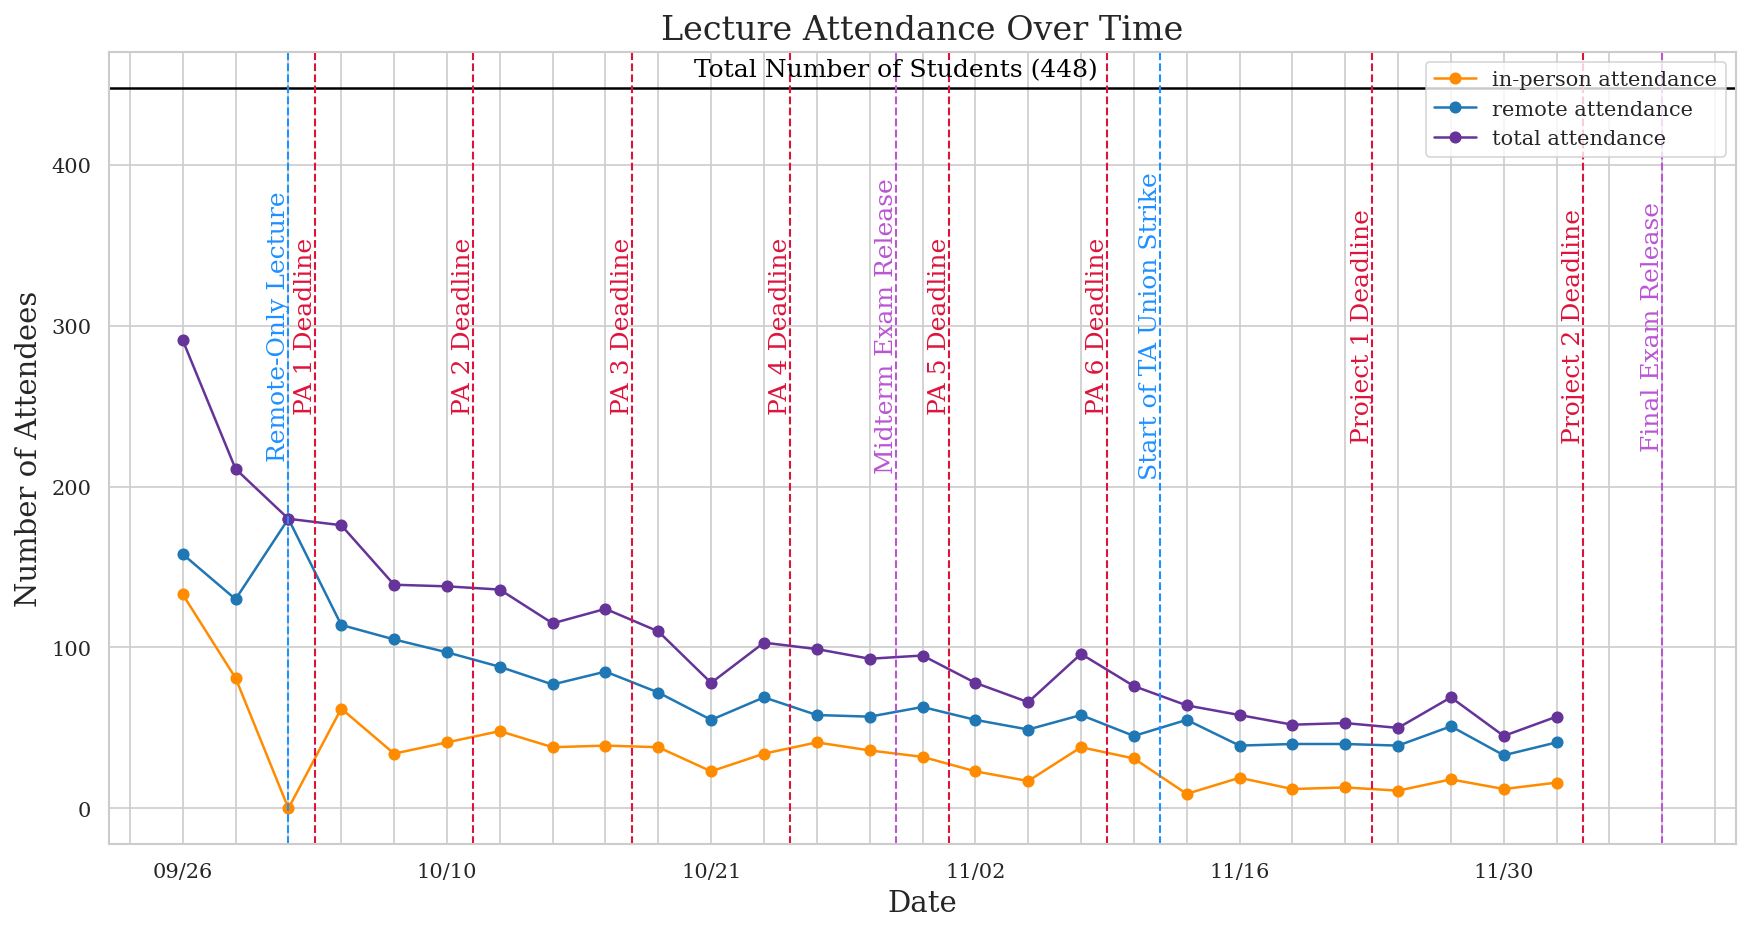
\includegraphics[width= 16cm]{figures/attendance_over_time.png}
    \caption{Synchronous attendance counts for the course lectures over time}
    \label{fig:attendance_over_time}
\end{figure}

As can be seen in Figure \ref{fig:attendance_over_time}, both in-person attendance and remote attendance gradually decreased over time, with certain events like the remote-only lecture and the start of the TA union strike having a noticeable correlation with each mode of attendance. In fact, those two events were the only points in the course other than the lecture after the midterm exam when the number of in-person attendees decreased and the number of remote attendees increased on the same day.

\section{Survey Results}

\subsection{Pre-Course Survey}

A total of 287 students submitted responses to the pre-course survey. For certain sections, the survey branched into separate questions for those it classified as hybrid/in-person attendees and those it classified as remote/asynchronous/non-attendees. Due to the low number of students who identified as a race that was not Asian or White, they were collectively classified as Other for the purposes of stratification. In addition, only a single student identified as a gender that was not male or female, so we limited our stratification based on gender to male and female students.

\begin{figure}[H]
    \vspace{5mm}
    \centering
    \textbf{In which section of the course are you officially enrolled? (N = 287)}\par\medskip
    \vspace{2mm}
    \begin{subfigure}[t]{1\textwidth}
        \centering
        \begin{tikzpicture}
            \begin{axis}[
                name=ax1,
                width=.4*\textwidth,
                height=9cm,
                major x tick style=transparent,
                ybar=2*\pgflinewidth,
                bar width=8pt,
                ymajorgrids=true,
                ylabel={Number of Responses},
                ylabel shift=-1mm,
                symbolic x coords={in-person,remote},
                xtick=data,
                x tick label style={
                    text width=6em,align=center,font=\small\linespread{0.8}\selectfont
                },
                scaled y ticks=false,
                enlarge x limits=.5,
                ymin=0,
                legend cell align=left,
                legend style={
                    at={(1.2,1.05)},
                    anchor=south,
                    column sep=1ex,
                    font=\footnotesize\linespread{.8}\selectfont,
                    /tikz/nodes={text width=4.5em,text height=.75em,text depth=,anchor=base},
                    align=left,
                    legend columns=5
                }
            ]
                \addplot[style={stand_1,fill=stand_1,mark=none}]
                    coordinates {(in-person,41) (remote,43)};
    
                \addplot[style={stand_2,fill=stand_2,mark=none}]
                    coordinates {(in-person,41) (remote,61)};
    
                \addplot[style={stand_3,fill=stand_3,mark=none}]
                    coordinates {(in-person,36) (remote,40)};
    
                \addplot[style={stand_4,fill=stand_4,mark=none}]
                    coordinates {(in-person,7) (remote,5)};
    
                \addplot[style={stand_5,fill=stand_5,mark=none}]
                    coordinates {(in-person,4) (remote,9)};

                \legend{2nd year,3rd year,4th year,5th+ year,Masters/PhD}
            \end{axis}at={(ax1.south east)},
            
            \begin{axis}[
                at={(ax1.south east)},
                xshift=2.5cm,
                width=.4*\textwidth,
                height=9cm,
                major x tick style=transparent,
                ybar=2*\pgflinewidth,
                bar width=8pt,
                ymajorgrids=true,
                ylabel={Percentage of Category},
                ylabel shift=-2mm,
                yticklabel={$\pgfmathprintnumber{\tick}\%$},
                ymin=0, ymax=100,
                extra y ticks={10,30,50,70,90},
                symbolic x coords={in-person,remote},
                xtick=data,
                x tick label style={
                    text width=6em,align=center,font=\small\linespread{0.8}\selectfont
                },
                scaled y ticks=false,
                enlarge x limits=.5,
                ymin=0,
            ]
                \addplot[style={stand_1,fill=stand_1,mark=none}]
                    coordinates {(in-person,48.81) (remote,51.19)};
    
                \addplot[style={stand_2,fill=stand_2,mark=none}]
                    coordinates {(in-person,40.20) (remote,59.80)};
    
                \addplot[style={stand_3,fill=stand_3,mark=none}]
                    coordinates {(in-person,47.37) (remote,52.63)};
    
                \addplot[style={stand_4,fill=stand_4,mark=none}]
                    coordinates {(in-person,58.33) (remote,41.67)};
    
                \addplot[style={stand_5,fill=stand_5,mark=none}]
                    coordinates {(in-person,30.77) (remote,69.23)};
            \end{axis}
        \end{tikzpicture}
        \caption{Stratified by class standing}
    \end{subfigure}
    \captionsetup{justification=centering}
    \caption{Number of respondents enrolled in each course section}
    \label{fig:enrollment_section}
\end{figure}

\begin{figure}[H]\ContinuedFloat
    \begin{subfigure}[t]{1\textwidth}
        \centering
        \begin{tikzpicture}
            \begin{axis}[
                name=ax1,
                width=.4*\textwidth,
                height=9cm,
                major x tick style=transparent,
                ybar=2*\pgflinewidth,
                bar width=8pt,
                ymajorgrids=true,
                ylabel={Number of Responses},
                ylabel shift=-1mm,
                symbolic x coords={in-person,remote},
                xtick=data,
                scaled y ticks=false,
                enlarge x limits=.5,
                ymin=0,
                legend cell align=left,
                legend style={
                    at={(1.2,1.05)},
                    anchor=south,
                    column sep=1ex,
                    font=\footnotesize\linespread{.8}\selectfont,
                    /tikz/nodes={text width=3em,text height=.75em,text depth=,anchor=base},
                    align=left,
                    legend columns=3
                }
            ]
                \addplot[style={race_1,fill=race_1,mark=none}]
                    coordinates {(in-person,21) (remote,29)};
    
                \addplot[style={race_2,fill=race_2,mark=none}]
                    coordinates {(in-person,100) (remote,128)};

                \addplot[style={race_3,fill=race_3,mark=none}]
                    coordinates {(in-person,8) (remote,12)};
                        
                \legend{White,Asian,Other}
            \end{axis}at={(ax1.south east)},
            
            \begin{axis}[
                at={(ax1.south east)},
                xshift=2.5cm,
                width=.4*\textwidth,
                height=9cm,
                major x tick style=transparent,
                ybar=2*\pgflinewidth,
                bar width=8pt,
                ymajorgrids=true,
                ylabel={Percentage of Category},
                ylabel shift=-2mm,
                yticklabel={$\pgfmathprintnumber{\tick}\%$},
                ymin=0, ymax=100,
                extra y ticks={10,30,50,70,90},
                symbolic x coords={in-person,remote},
                xtick=data,
                scaled y ticks=false,
                enlarge x limits=.5,
                ymin=0,
            ]
                \addplot[style={race_1,fill=race_1,mark=none}]
                    coordinates {(in-person,42.00) (remote,58.00)};
    
                \addplot[style={race_2,fill=race_2,mark=none}]
                    coordinates {(in-person,43.86) (remote,56.14)};
    
                \addplot[style={race_3,fill=race_3,mark=none}]
                    coordinates {(in-person,40.00) (remote,60.00)};
            \end{axis}
        \end{tikzpicture}
        \caption{Stratified by race}
    \end{subfigure}
    
    \begin{subfigure}[t]{1\textwidth}
        \vspace{5mm}
        \centering
        \begin{tikzpicture}
            \begin{axis}[
                name=ax1,
                width=.4*\textwidth,
                height=9cm,
                major x tick style=transparent,
                ybar=2*\pgflinewidth,
                bar width=8pt,
                ymajorgrids=true,
                ylabel={Number of Responses},
                ylabel shift=-1mm,
                symbolic x coords={in-person,remote},
                xtick=data,
                scaled y ticks=false,
                enlarge x limits=.5,
                ymin=0,
                legend cell align=left,
                legend style={
                    at={(1.2,1.05)},
                    anchor=south,
                    column sep=1ex,
                    font=\footnotesize\linespread{.8}\selectfont,
                    /tikz/nodes={text width=3em,text height=.75em,text depth=,anchor=base},
                    align=left,
                    legend columns=2
                }
            ]
                \addplot[style={gender_1,fill=gender_1,mark=none}]
                    coordinates {(in-person,86) (remote,124)};
    
                \addplot[style={gender_2,fill=gender_2,mark=none}]
                    coordinates {(in-person,40) (remote,31)};
        
                \legend{Male,Female}
            \end{axis}at={(ax1.south east)},
            
            \begin{axis}[
                at={(ax1.south east)},
                xshift=2.5cm,
                width=.4*\textwidth,
                height=9cm,
                major x tick style=transparent,
                ybar=2*\pgflinewidth,
                bar width=8pt,
                ymajorgrids=true,
                ylabel={Percentage of Category},
                ylabel shift=-2mm,
                yticklabel={$\pgfmathprintnumber{\tick}\%$},
                ymin=0, ymax=100,
                extra y ticks={10,30,50,70,90},
                symbolic x coords={in-person,remote},
                xtick=data,
                scaled y ticks=false,
                enlarge x limits=.5,
                ymin=0,
            ]
                \addplot[style={gender_1,fill=gender_1,mark=none}]
                    coordinates {(in-person,40.95) (remote,59.05)};
    
                \addplot[style={gender_2,fill=gender_2,mark=none}]
                    coordinates {(in-person,56.34) (remote,43.66)};
            \end{axis}
        \end{tikzpicture}
        \caption{Stratified by gender}
    \end{subfigure}
    \captionsetup{justification=centering}
    \caption[]{Number of respondents enrolled in each course section (cont.)}
\end{figure}

Students were asked to state which section they were enrolled in at the start of the course. Given that there were 189 students enrolled in the in-person section and 203 students enrolled in the remote section overall, 44.95\% of respondents were in-person enrollees, while 55.05\% were remote enrollees. In the days leading up to the enrollment deadline, we found that some students remained on the waitlist for the in-person section even while there were seats available in the remote section, despite the fact that they were identical in all but name.

When we stratify course enrollment by class standing, we see that third-year students made up a higher percentage of the enrollment for the remote section than the in-person section, at 38.6\% and 31.8\%. Other than this, however, enrollment was fairly even across the two sections. Neither race nor gender appeared to have a significant impact on a student's section of enrollment.

\begin{figure}[H]
    \vspace{5mm}
    \centering
    \textbf{Why did you choose to enroll in the in-person section? (N = 129)}\par\medskip
    \vspace{2mm}
    \begin{subfigure}[t]{1\textwidth}
        \centering
        \begin{tikzpicture}
            \begin{axis}[
                width=.85*\textwidth,
                height=9cm,
                major x tick style=transparent,
                ybar=2*\pgflinewidth,
                bar width=8pt,
                ymajorgrids=true,
                ylabel={Number of Responses},
                symbolic x coords={prefer in-person,easier to learn in-person,will already be on campus,will be unable to focus if remote},
                xtick=data,
                x tick label style={
                    text width=6em,align=center,font=\footnotesize\linespread{0.8}\selectfont
                },
                scaled y ticks=false,
                enlarge x limits=.25,
                ymin=0,
                legend cell align=left,
                legend style={
                    at={(.5,1.05)},
                    anchor=south,
                    column sep=1ex,
                    font=\footnotesize\linespread{.8}\selectfont,
                    /tikz/nodes={text width=4.5em,text height=.75em,text depth=,anchor=base},
                    align=left,
                    legend columns=5
                }
            ]
                \addplot[style={stand_1,fill=stand_1,mark=none}]
                coordinates {(prefer in-person,28) (easier to learn in-person,18) (will already be on campus,26) (will be unable to focus if remote,25)};

                \addplot[style={stand_2,fill=stand_2,mark=none}]
                    coordinates {(prefer in-person,19) (easier to learn in-person,18) (will already be on campus,15) (will be unable to focus if remote,21)};
    
                \addplot[style={stand_3,fill=stand_3,mark=none}]
                    coordinates {(prefer in-person,23) (easier to learn in-person,19) (will already be on campus,20) (will be unable to focus if remote,17)};
    
                \addplot[style={stand_4,fill=stand_4,mark=none}]
                    coordinates {(prefer in-person,4) (easier to learn in-person,4) (will already be on campus,1) (will be unable to focus if remote,5)};
    
                \addplot[style={stand_5,fill=stand_5,mark=none}]
                    coordinates {(prefer in-person,2) (easier to learn in-person,0) (will already be on campus,0) (will be unable to focus if remote,1)};
        
                \legend{2nd year,3rd year,4th year,5th+ year,Masters/PhD}
            \end{axis}
        
            \begin{axis}[
                yshift=-9cm,
                width=.85*\textwidth,
                height=9cm,
                major x tick style=transparent,
                ybar=2*\pgflinewidth,
                bar width=8pt,
                ymajorgrids=true,
                ylabel={Percentage of Category},
                ylabel shift=-2mm,
                yticklabel={$\pgfmathprintnumber{\tick}\%$},
                ymin=0, ymax=100,
                extra y ticks={10,30,50,70,90},
                symbolic x coords={prefer in-person,easier to learn in-person,will already be on campus,will be unable to focus if remote},
                xtick=data,
                x tick label style={
                    text width=6em,align=center,font=\footnotesize\linespread{0.8}\selectfont
                },
                scaled y ticks=false,
                enlarge x limits=.25,
                ymin=0,
            ]            
                \addplot[style={stand_1,fill=stand_1,mark=none}]
                coordinates {(prefer in-person,68.29) (easier to learn in-person,43.90) (will already be on campus,63.41) (will be unable to focus if remote,60.98)};

                \addplot[style={stand_2,fill=stand_2,mark=none}]
                    coordinates {(prefer in-person,46.34) (easier to learn in-person,43.90) (will already be on campus,36.59) (will be unable to focus if remote,51.22)};
    
                \addplot[style={stand_3,fill=stand_3,mark=none}]
                    coordinates {(prefer in-person,63.89) (easier to learn in-person,52.78) (will already be on campus,55.56) (will be unable to focus if remote,47.22)};
    
                \addplot[style={stand_4,fill=stand_4,mark=none}]
                    coordinates {(prefer in-person,57.14) (easier to learn in-person,57.14) (will already be on campus,14.29) (will be unable to focus if remote,71.43)};
    
                \addplot[style={stand_5,fill=stand_5,mark=none}]
                    coordinates {(prefer in-person,50.00) (easier to learn in-person,0.00) (will already be on campus,0.00) (will be unable to focus if remote,25.00)};
            \end{axis}
        \end{tikzpicture}
        \caption{Stratified by class standing}
    \end{subfigure}
    \captionsetup{justification=centering}
    \caption{Reasons why respondents enrolled in the in-person section}
    \label{fig:inperson_enrollment_reasons}
\end{figure}

\begin{figure}[H]\ContinuedFloat
    \centering
    \begin{subfigure}[t]{1\textwidth}
        \vspace{5mm}
        \centering
        \begin{tikzpicture}
            \begin{axis}[
                width=.9*\textwidth,
                height=9cm,
                major x tick style=transparent,
                ybar=2*\pgflinewidth,
                bar width=8pt,
                ymajorgrids=true,
                ylabel={Number of Responses},
                symbolic x coords={prefer in-person,easier to learn in-person,will already be on campus,will be unable to focus if remote},
                xtick=data,
                x tick label style={
                    text width=6em,align=center,font=\footnotesize\linespread{0.8}\selectfont
                },
                scaled y ticks=false,
                enlarge x limits=.15,
                ymin=0,
                legend cell align=left,
                legend style={
                    at={(.5,1.05)},
                    anchor=south,
                    column sep=1ex,
                    font=\footnotesize\linespread{.8}\selectfont,
                    /tikz/nodes={text width=3em,text height=.75em,text depth=,anchor=base},
                    align=left,
                    legend columns=3
                }
            ]
                \addplot[style={race_1,fill=race_1,mark=none}]
                coordinates {(prefer in-person,15) (easier to learn in-person,12) (will already be on campus,12) (will be unable to focus if remote,11)};
    
                \addplot[style={race_2,fill=race_2,mark=none}]
                coordinates {(prefer in-person,54) (easier to learn in-person,43) (will already be on campus,46) (will be unable to focus if remote,53)};
    
                \addplot[style={race_3,fill=race_3,mark=none}]
                coordinates {(prefer in-person,6) (easier to learn in-person,3) (will already be on campus,5) (will be unable to focus if remote,4)};
        
                \legend{White,Asian,Other}
            \end{axis}
        
            \begin{axis}[
                yshift=-9cm,
                width=.9*\textwidth,
                height=9cm,
                major x tick style=transparent,
                ybar=2*\pgflinewidth,
                bar width=8pt,
                ymajorgrids=true,
                ylabel={Percentage of Category},
                ylabel shift=-2mm,
                yticklabel={$\pgfmathprintnumber{\tick}\%$},
                ymin=0, ymax=100,
                extra y ticks={10,30,50,70,90},
                symbolic x coords={prefer in-person,easier to learn in-person,will already be on campus,will be unable to focus if remote},
                xtick=data,
                x tick label style={
                    text width=6em,align=center,font=\footnotesize\linespread{0.8}\selectfont
                },
                scaled y ticks=false,
                enlarge x limits=.15,
                ymin=0,
            ]
                \addplot[style={race_1,fill=race_1,mark=none}]
                coordinates {(prefer in-person,71.43) (easier to learn in-person,57.14) (will already be on campus,57.14) (will be unable to focus if remote,52.38)};
    
                \addplot[style={race_2,fill=race_2,mark=none}]
                coordinates {(prefer in-person,54.00) (easier to learn in-person,43.00) (will already be on campus,46.00) (will be unable to focus if remote,53.00)};
    
                \addplot[style={race_3,fill=race_3,mark=none}]
                coordinates {(prefer in-person,75.00) (easier to learn in-person,37.5) (will already be on campus,62.5) (will be unable to focus if remote,50.00)};
            \end{axis}
        \end{tikzpicture}
        \caption{Stratified by race}
    \end{subfigure}
    \captionsetup{justification=centering}
    \caption[]{Reasons why respondents enrolled in the in-person section (cont.)}
\end{figure}

\begin{figure}[H]\ContinuedFloat
    \centering
    \begin{subfigure}[t]{1\textwidth}
        \centering
        \begin{tikzpicture}
            \begin{axis}[
                width=.9*\textwidth,
                height=9cm,
                major x tick style=transparent,
                ybar=2*\pgflinewidth,
                bar width=8pt,
                ymajorgrids=true,
                ylabel={Number of Responses},
                symbolic x coords={prefer in-person,easier to learn in-person,will already be on campus,will be unable to focus if remote},
                xtick=data,
                x tick label style={
                    text width=6em,align=center,font=\footnotesize\linespread{0.8}\selectfont
                },
                scaled y ticks=false,
                enlarge x limits=.15,
                ymin=0,
                legend cell align=left,
                legend style={
                    at={(.5,1.05)},
                    anchor=south,
                    column sep=1ex,
                    font=\footnotesize\linespread{.8}\selectfont,
                    /tikz/nodes={text width=3em,text height=.75em,text depth=,anchor=base},
                    align=left,
                    legend columns=2
                }
            ]
                \addplot[style={gender_1,fill=gender_1,mark=none}]
                coordinates {(prefer in-person,52) (easier to learn in-person,39) (will already be on campus,42) (will be unable to focus if remote,44)};
    
                \addplot[style={gender_2,fill=gender_2,mark=none}]
                coordinates {(prefer in-person,21) (easier to learn in-person,19) (will already be on campus,19) (will be unable to focus if remote,23)};
        
                \legend{Male,Female}
            \end{axis},
            
            \begin{axis}[
                yshift=-9cm,
                width=.9*\textwidth,
                height=9cm,
                major x tick style=transparent,
                ybar=2*\pgflinewidth,
                bar width=8pt,
                ymajorgrids=true,
                ylabel={Percentage of Category},
                ylabel shift=-2mm,
                yticklabel={$\pgfmathprintnumber{\tick}\%$},
                ymin=0, ymax=100,
                extra y ticks={10,30,50,70,90},
                symbolic x coords={prefer in-person,easier to learn in-person,will already be on campus,will be unable to focus if remote},
                xtick=data,
                x tick label style={
                    text width=6em,align=center,font=\footnotesize\linespread{0.8}\selectfont
                },
                scaled y ticks=false,
                enlarge x limits=.15,
                ymin=0,
            ]
                \addplot[style={gender_1,fill=gender_1,mark=none}]
                coordinates {(prefer in-person,60.47) (easier to learn in-person,45.35) (will already be on campus,48.84) (will be unable to focus if remote,51.16)};
    
                \addplot[style={gender_2,fill=gender_2,mark=none}]
                coordinates {(prefer in-person,52.5) (easier to learn in-person,47.5) (will already be on campus,47.5) (will be unable to focus if remote,57.5)};
            \end{axis}
        \end{tikzpicture}
        \caption{Stratified by gender}
    \end{subfigure}
    \captionsetup{justification=centering}
    \caption[]{Reasons why respondents enrolled in the in-person section (cont.)}
    \vspace{10mm}
\end{figure}

129 of the pre-course survey respondents were enrolled in the in-person section. When asked why they did so, 58.9\% stated that they preferred to learn in an in-person environment, 45.7\% stated that they found it easier to learn in person, 48.1\% stated that they would already be on campus when lectures took place, and 53.5\% expressed concern that they would be unable to focus if they attended remotely (see Figure \ref{fig:inperson_enrollment_reasons}). Though only about half of the respondents selected each of the available reasons, the fact that at least one of these reasons was selected by every respondent enrolled in the in-person section shows that they did so out of some level of preference for in-person instruction over remote instruction.

When we stratify by class standing, we see that the second-year students were most likely to find the in-person section convenient due to already being on campus. We expected this to be the case, since on-campus housing is only guaranteed for undergraduate students up to the end of their second year of enrollment. Other than this, however, the reasons were fairly proportional with class standing. In addition, reasons were even across students of different races and genders.

% When in-person enrollees were asked how often they planned to attend lectures in person, 69.0\% said they would attend as often as possible (i.e., three times a week). This indicates that, while actual in-person attendance was much lower, a majority of students in the in-person section had intended to engage with the in-person modality of the course when they started.

\begin{figure}[H]
    \vspace{5mm}
    \centering
    \textbf{Why did you choose to enroll in the remote section? (N = 158)}\par\medskip
    \vspace{2mm}
    \begin{subfigure}[t]{1\textwidth}
        \centering
        \begin{tikzpicture}
            \begin{axis}[
                width=.85*\textwidth,
                height=9cm,
                major x tick style=transparent,
                ybar=2*\pgflinewidth,
                bar width=8pt,
                ymajorgrids=true,
                ylabel={Number of Responses},
                symbolic x coords={prefer remote,easier to learn remote,unable to get to campus,concerned for health,in-person section was full},
                xtick=data,
                x tick label style={
                    text width=6em,align=center,font=\footnotesize\linespread{0.8}\selectfont
                },
                scaled y ticks=false,
                enlarge x limits=.25,
                ymin=0,
                legend cell align=left,
                legend style={
                    at={(.5,1.05)},
                    anchor=south,
                    column sep=1ex,
                    font=\footnotesize\linespread{.8}\selectfont,
                    /tikz/nodes={text width=4.5em,text height=.75em,text depth=,anchor=base},
                    align=left,
                    legend columns=5
                }
            ]
                \addplot[style={stand_1,fill=stand_1,mark=none}]
                    coordinates {(prefer remote,15) (easier to learn remote,7) (unable to get to campus,3) (concerned for health,2) (in-person section was full,31)};
    
                \addplot[style={stand_2,fill=stand_2,mark=none}]
                    coordinates {(prefer remote,21) (easier to learn remote,20) (unable to get to campus,13) (concerned for health,7) (in-person section was full,36)};
    
                \addplot[style={stand_3,fill=stand_3,mark=none}]
                    coordinates {(prefer remote,19) (easier to learn remote,14) (unable to get to campus,12) (concerned for health,6) (in-person section was full,21)};
    
                \addplot[style={stand_4,fill=stand_4,mark=none}]
                    coordinates {(prefer remote,2) (easier to learn remote,1) (unable to get to campus,3) (concerned for health,0) (in-person section was full,2)};
    
                \addplot[style={stand_5,fill=stand_5,mark=none}]
                    coordinates {(prefer remote,5) (easier to learn remote,2) (unable to get to campus,1) (concerned for health,0) (in-person section was full,7)};
        
                \legend{2nd year,3rd year,4th year,5th+ year,Masters/PhD}
            \end{axis}
        
            \begin{axis}[
                yshift=-9cm,
                width=.85*\textwidth,
                height=9cm,
                major x tick style=transparent,
                ybar=2*\pgflinewidth,
                bar width=8pt,
                ymajorgrids=true,
                ylabel={Percentage of Category},
                ylabel shift=-2mm,
                yticklabel={$\pgfmathprintnumber{\tick}\%$},
                ymin=0, ymax=100,
                extra y ticks={10,30,50,70,90},
                symbolic x coords={prefer remote,easier to learn remote,unable to get to campus,concerned for health,in-person section was full},
                xtick=data,
                x tick label style={
                    text width=6em,align=center,font=\footnotesize\linespread{0.8}\selectfont
                },
                scaled y ticks=false,
                enlarge x limits=.25,
                ymin=0,
            ]            
                \addplot[style={stand_1,fill=stand_1,mark=none}]
                    coordinates {(prefer remote,34.88) (easier to learn remote,16.28) (unable to get to campus,6.98) (concerned for health,4.65) (in-person section was full,72.09)};
    
                \addplot[style={stand_2,fill=stand_2,mark=none}]
                    coordinates {(prefer remote,34.43) (easier to learn remote,32.79) (unable to get to campus,21.31) (concerned for health,11.48) (in-person section was full,59.02)};
    
                \addplot[style={stand_3,fill=stand_3,mark=none}]
                    coordinates {(prefer remote,47.50) (easier to learn remote,35.00) (unable to get to campus,30.00) (concerned for health,15.00) (in-person section was full,52.50)};
    
                \addplot[style={stand_4,fill=stand_4,mark=none}]
                    coordinates {(prefer remote,40.00) (easier to learn remote,20.00) (unable to get to campus,60.00) (concerned for health,0.00) (in-person section was full,40.00)};
    
                \addplot[style={stand_5,fill=stand_5,mark=none}]
                    coordinates {(prefer remote,55.56) (easier to learn remote,22.22) (unable to get to campus,11.11) (concerned for health,0.00) (in-person section was full,77.78)};
            \end{axis}
        \end{tikzpicture}
        \caption{Stratified by class standing}
    \end{subfigure}
    \captionsetup{justification=centering}
    \caption{Reasons why respondents enrolled in the remote section}
    \label{fig:remote_enrollment_reasons}
\end{figure}

\begin{figure}[H]\ContinuedFloat
    \centering
    \begin{subfigure}[t]{1\textwidth}
        \vspace{5mm}
        \centering
        \begin{tikzpicture}
            \begin{axis}[
                width=.9*\textwidth,
                height=9cm,
                major x tick style=transparent,
                ybar=2*\pgflinewidth,
                bar width=8pt,
                ymajorgrids=true,
                ylabel={Number of Responses},
                symbolic x coords={prefer remote,easier to learn remote,unable to get to campus,concerned for health,in-person section was full},
                xtick=data,
                x tick label style={
                    text width=6em,align=center,font=\footnotesize\linespread{0.8}\selectfont
                },
                scaled y ticks=false,
                enlarge x limits=.15,
                ymin=0,
                legend cell align=left,
                legend style={
                    at={(.5,1.05)},
                    anchor=south,
                    column sep=1ex,
                    font=\footnotesize\linespread{.8}\selectfont,
                    /tikz/nodes={text width=3em,text height=.75em,text depth=,anchor=base},
                    align=left,
                    legend columns=3
                }
            ]
                \addplot[style={race_1,fill=race_1,mark=none}]
                    coordinates {(prefer remote,11) (easier to learn remote,6) (unable to get to campus,5) (concerned for health,1) (in-person section was full,20)};
        
                \addplot[style={race_2,fill=race_2,mark=none}]
                    coordinates {(prefer remote,52) (easier to learn remote,38) (unable to get to campus,26) (concerned for health,14) (in-person section was full,78)};
    
                \addplot[style={race_3,fill=race_3,mark=none}]
                    coordinates {(prefer remote,3) (easier to learn remote,2) (unable to get to campus,3) (concerned for health,0) (in-person section was full,6)};
    
                \legend{White,Asian,Other}
            \end{axis}
        
            \begin{axis}[
                yshift=-9cm,
                width=.9*\textwidth,
                height=9cm,
                major x tick style=transparent,
                ybar=2*\pgflinewidth,
                bar width=8pt,
                ymajorgrids=true,
                ylabel={Percentage of Category},
                ylabel shift=-2mm,
                yticklabel={$\pgfmathprintnumber{\tick}\%$},
                ymin=0, ymax=100,
                extra y ticks={10,30,50,70,90},
                symbolic x coords={prefer remote,easier to learn remote,unable to get to campus,concerned for health,in-person section was full},
                xtick=data,
                x tick label style={
                    text width=6em,align=center,font=\footnotesize\linespread{0.8}\selectfont
                },
                scaled y ticks=false,
                enlarge x limits=.15,
                ymin=0,
            ]
                \addplot[style={race_1,fill=race_1,mark=none}]
                    coordinates {(prefer remote,37.93) (easier to learn remote,20.69) (unable to get to campus,17.24) (concerned for health,3.45) (in-person section was full,68.97)};
        
                \addplot[style={race_2,fill=race_2,mark=none}]
                    coordinates {(prefer remote,40.63) (easier to learn remote,29.69) (unable to get to campus,20.31) (concerned for health,10.94) (in-person section was full,60.94)};
    
                \addplot[style={race_3,fill=race_3,mark=none}]
                    coordinates {(prefer remote,33.33) (easier to learn remote,22.22) (unable to get to campus,33.33) (concerned for health,0.00) (in-person section was full,66.67)};
            \end{axis}
        \end{tikzpicture}
        \caption{Stratified by race}
    \end{subfigure}
    \captionsetup{justification=centering}
    \caption[]{Reasons why respondents enrolled in the remote section (cont.)}
\end{figure}

\begin{figure}[H]\ContinuedFloat
    \centering
    \begin{subfigure}[t]{1\textwidth}
        \centering
        \begin{tikzpicture}
            \begin{axis}[
                width=.9*\textwidth,
                height=9cm,
                major x tick style=transparent,
                ybar=2*\pgflinewidth,
                bar width=8pt,
                ymajorgrids=true,
                ylabel={Number of Responses},
                symbolic x coords={prefer remote,easier to learn remote,unable to get to campus,concerned for health,in-person section was full},
                xtick=data,
                x tick label style={
                    text width=6em,align=center,font=\footnotesize\linespread{0.8}\selectfont
                },
                scaled y ticks=false,
                enlarge x limits=.15,
                ymin=0,
                legend cell align=left,
                legend style={
                    at={(.5,1.05)},
                    anchor=south,
                    column sep=1ex,
                    font=\footnotesize\linespread{.8}\selectfont,
                    /tikz/nodes={text width=3em,text height=.75em,text depth=,anchor=base},
                    align=left,
                    legend columns=2
                }
            ]
                \addplot[style={gender_1,fill=gender_1,mark=none}]
                    coordinates {(prefer remote,55) (easier to learn remote,39) (unable to get to campus,24) (concerned for health,14) (in-person section was full,75)};
    
                \addplot[style={gender_2,fill=gender_2,mark=none}]
                    coordinates {(prefer remote,6) (easier to learn remote,4) (unable to get to campus,7) (concerned for health,0) (in-person section was full,20)};
        
                \legend{Male,Female}
            \end{axis},
            
            \begin{axis}[
                yshift=-9cm,
                width=.9*\textwidth,
                height=9cm,
                major x tick style=transparent,
                ybar=2*\pgflinewidth,
                bar width=8pt,
                ymajorgrids=true,
                ylabel={Percentage of Category},
                ylabel shift=-2mm,
                yticklabel={$\pgfmathprintnumber{\tick}\%$},
                ymin=0, ymax=100,
                extra y ticks={10,30,50,70,90},
                symbolic x coords={prefer remote,easier to learn remote,unable to get to campus,concerned for health,in-person section was full},
                xtick=data,
                x tick label style={
                    text width=6em,align=center,font=\footnotesize\linespread{0.8}\selectfont
                },
                scaled y ticks=false,
                enlarge x limits=.15,
                ymin=0,
            ]
                \addplot[style={gender_1,fill=gender_1,mark=none}]
                    coordinates {(prefer remote,44.35) (easier to learn remote,31.45) (unable to get to campus,19.35) (concerned for health,11.29) (in-person section was full,60.48)};
    
                \addplot[style={gender_2,fill=gender_2,mark=none}]
                    coordinates {(prefer remote,19.35) (easier to learn remote,12.90) (unable to get to campus,22.58) (concerned for health,0.00) (in-person section was full,64.52)};
            \end{axis}
        \end{tikzpicture}
        \caption{Stratified by gender}
    \end{subfigure}
    \captionsetup{justification=centering}
    \caption[]{Reasons why respondents enrolled in the remote section (cont.)}
    \vspace{10mm}
\end{figure}

158 of the pre-course survey respondents were enrolled in the remote section. When asked why they did so, 39.2\% stated that they preferred to learn in a remote environment, 27.8\% stated that they found it easier to learn remotely, 20.3\% stated that they would be unable to get to campus for the lectures, and 61.4\% stated that they did so simply because the in-person section was full (see Figure \ref{fig:remote_enrollment_reasons}). By a large margin, the most common reason that students had enrolled in the remote section was because they were unable to enroll in the in-person section. This may have been due to the fact that the remote section was listed under a new course code and therefore made students unsure as to whether it would fulfill the same requirements as the in-person section.

When we stratify students' reasons for remote section enrollment by their class standing, we see further evidence that students were hesitant to enroll in the remote section due to the new course code: proportionally, second-year undergraduate students and graduate students were more likely than students of other class standings to indicate that they had done so because the in-person section was full. Students who were earlier on in their undergraduate degree may have been more cautious about whether their requirements would be met because this course is a prerequisite to many other upper-division courses in the department, making it a critical requirement for students in their second year. Meanwhile, graduate students may have also been more cautious about enrolling in the in-person section because they were unsure whether the remote section would fulfill their elective requirement. Stratifying by race does not reveal any significant differences in reasoning across students of different races; however, stratifying by gender reveals that male students are twice as likely to prefer remote courses and find it easy to learn in remote courses as female students.

% Remote enrollees were asked whether they planned to attend an in-person lecture at some point during the course: 47.5\% said that they did, 12.0\% said that they did not, and 40.5\% said that they were not yet sure. This matches the previous responses indicating that many students were only enrolled in the remote section because the in-person section was full.

\begin{figure}[H]
    \vspace{5mm}
    \centering
    \textbf{If this course was only offered as either an in-person or a remote course, which modality would you prefer? (N = 287)}\par\medskip
    \vspace{2mm}
    \begin{subfigure}[t]{1\textwidth}
        \centering
        \begin{tikzpicture}
            \begin{axis}[
                width=.7*\textwidth,
                height=9cm,
                major x tick style=transparent,
                ybar=2*\pgflinewidth,
                bar width=8pt,
                ymajorgrids=true,
                ylabel={Number of Responses},
                symbolic x coords={in-person,remote,neither},
                xtick=data,
                x tick label style={
                    text width=6em,align=center,font=\footnotesize\linespread{0.8}\selectfont
                },
                scaled y ticks=false,
                enlarge x limits=.25,
                ymin=0,
                legend cell align=left,
                legend style={
                    at={(.5,1.05)},
                    anchor=south,
                    column sep=1ex,
                    font=\footnotesize\linespread{.8}\selectfont,
                    /tikz/nodes={text width=4.5em,text height=.75em,text depth=,anchor=base},
                    align=left,
                    legend columns=5
                }
            ]
                \addplot[style={stand_1,fill=stand_1,mark=none}]
                    coordinates {(in-person,43) (remote,24) (neither,17)};

                \addplot[style={stand_2,fill=stand_2,mark=none}]
                    coordinates {(in-person,39) (remote,41) (neither,22)};
    
                \addplot[style={stand_3,fill=stand_3,mark=none}]
                    coordinates {(in-person,24) (remote,33) (neither,19)};
    
                \addplot[style={stand_4,fill=stand_4,mark=none}]
                    coordinates {(in-person,5) (remote,6) (neither,1)};
    
                \addplot[style={stand_5,fill=stand_5,mark=none}]
                    coordinates {(in-person,1) (remote,10) (neither,2)};
        
                \legend{2nd year,3rd year,4th year,5th+ year,Masters/PhD}
            \end{axis}
        
            \begin{axis}[
                yshift=-9cm,
                width=.7*\textwidth,
                height=9cm,
                major x tick style=transparent,
                ybar=2*\pgflinewidth,
                bar width=8pt,
                ymajorgrids=true,
                ylabel={Percentage of Category},
                ylabel shift=-2mm,
                yticklabel={$\pgfmathprintnumber{\tick}\%$},
                ymin=0, ymax=100,
                extra y ticks={10,30,50,70,90},
                symbolic x coords={in-person,remote,neither},
                xtick=data,
                x tick label style={
                    text width=6em,align=center,font=\footnotesize\linespread{0.8}\selectfont
                },
                scaled y ticks=false,
                enlarge x limits=.25,
                ymin=0,
            ]            
                \addplot[style={stand_1,fill=stand_1,mark=none}]
                    coordinates {(in-person,51.19) (remote,28.57) (neither,20.24)};

                \addplot[style={stand_2,fill=stand_2,mark=none}]
                    coordinates {(in-person,38.24) (remote,40.20) (neither,21.57)};
    
                \addplot[style={stand_3,fill=stand_3,mark=none}]
                    coordinates {(in-person,31.58) (remote,43.42) (neither,25.00)};
    
                \addplot[style={stand_4,fill=stand_4,mark=none}]
                    coordinates {(in-person,41.67) (remote,50.00) (neither,8.33)};
    
                \addplot[style={stand_5,fill=stand_5,mark=none}]
                    coordinates {(in-person,7.69) (remote,76.92) (neither,15.38)};
            \end{axis}
        \end{tikzpicture}
        \caption{Stratified by class standing}
    \end{subfigure}
    \captionsetup{justification=centering}
    \caption{Respondents who would have preferred either an in-person or a remote course}
    \label{fig:modality_preference}
\end{figure}

\begin{figure}[H]\ContinuedFloat
    \centering
    \begin{subfigure}[t]{1\textwidth}
        \vspace{5mm}
        \centering
        \begin{tikzpicture}
            \begin{axis}[
                width=.6*\textwidth,
                height=9cm,
                major x tick style=transparent,
                ybar=2*\pgflinewidth,
                bar width=8pt,
                ymajorgrids=true,
                ylabel={Number of Responses},
                symbolic x coords={in-person,remote,neither},
                xtick=data,
                x tick label style={
                    text width=6em,align=center,font=\footnotesize\linespread{0.8}\selectfont
                },
                scaled y ticks=false,
                enlarge x limits=.25,
                ymin=0,
                legend cell align=left,
                legend style={
                    at={(.5,1.05)},
                    anchor=south,
                    column sep=1ex,
                    font=\footnotesize\linespread{.8}\selectfont,
                    /tikz/nodes={text width=3em,text height=.75em,text depth=,anchor=base},
                    align=left,
                    legend columns=3
                }
            ]
                \addplot[style={race_1,fill=race_1,mark=none}]
                    coordinates {(in-person,28) (remote,13) (neither,9)};

                \addplot[style={race_2,fill=race_2,mark=none}]
                    coordinates {(in-person,80) (remote,98) (neither,50)};

                \addplot[style={race_3,fill=race_3,mark=none}]
                    coordinates {(in-person,6) (remote,8) (neither,3)};

                \legend{White,Asian,Other}
            \end{axis}
        
            \begin{axis}[
                yshift=-9cm,
                width=.6*\textwidth,
                height=9cm,
                major x tick style=transparent,
                ybar=2*\pgflinewidth,
                bar width=8pt,
                ymajorgrids=true,
                ylabel={Percentage of Category},
                ylabel shift=-2mm,
                yticklabel={$\pgfmathprintnumber{\tick}\%$},
                ymin=0, ymax=100,
                extra y ticks={10,30,50,70,90},
                symbolic x coords={in-person,remote,neither},
                xtick=data,
                x tick label style={
                    text width=6em,align=center,font=\footnotesize\linespread{0.8}\selectfont
                },
                scaled y ticks=false,
                enlarge x limits=.25,
                ymin=0,
            ]
                \addplot[style={race_1,fill=race_1,mark=none}]
                    coordinates {(in-person,56.00) (remote,26.00) (neither,18.00)};

                \addplot[style={race_2,fill=race_2,mark=none}]
                    coordinates {(in-person,35.09) (remote,42.98) (neither,21.93)};

                \addplot[style={race_3,fill=race_3,mark=none}]
                    coordinates {(in-person,35.29) (remote,47.06) (neither,17.65)};
            \end{axis}
        \end{tikzpicture}
        \caption{Stratified by race}
    \end{subfigure}
    \captionsetup{justification=centering}
    \caption[]{Respondents who would have preferred either an in-person or a remote course (cont.)}
\end{figure}

\begin{figure}[H]\ContinuedFloat
    \centering
    \begin{subfigure}[t]{1\textwidth}
        \centering
        \begin{tikzpicture}
            \begin{axis}[
                width=.6*\textwidth,
                height=9cm,
                major x tick style=transparent,
                ybar=2*\pgflinewidth,
                bar width=8pt,
                ymajorgrids=true,
                ylabel={Number of Responses},
                symbolic x coords={in-person,remote,neither},
                xtick=data,
                x tick label style={
                    text width=6em,align=center,font=\footnotesize\linespread{0.8}\selectfont
                },
                scaled y ticks=false,
                enlarge x limits=.25,
                ymin=0,
                legend cell align=left,
                legend style={
                    at={(.5,1.05)},
                    anchor=south,
                    column sep=1ex,
                    font=\footnotesize\linespread{.8}\selectfont,
                    /tikz/nodes={text width=3em,text height=.75em,text depth=,anchor=base},
                    align=left,
                    legend columns=2
                }
            ]
                \addplot[style={gender_1,fill=gender_1,mark=none}]
                    coordinates {(in-person,74) (remote,96) (neither,40)};
    
                \addplot[style={gender_2,fill=gender_2,mark=none}]
                    coordinates {(in-person,35) (remote,17) (neither,19)};
        
                \legend{Male,Female}
            \end{axis},
            
            \begin{axis}[
                yshift=-9cm,
                width=.6*\textwidth,
                height=9cm,
                major x tick style=transparent,
                ybar=2*\pgflinewidth,
                bar width=8pt,
                ymajorgrids=true,
                ylabel={Percentage of Category},
                ylabel shift=-2mm,
                yticklabel={$\pgfmathprintnumber{\tick}\%$},
                ymin=0, ymax=100,
                extra y ticks={10,30,50,70,90},
                symbolic x coords={in-person,remote,neither},
                xtick=data,
                x tick label style={
                    text width=6em,align=center,font=\footnotesize\linespread{0.8}\selectfont
                },
                scaled y ticks=false,
                enlarge x limits=.25,
                ymin=0,
            ]
                \addplot[style={gender_1,fill=gender_1,mark=none}]
                    coordinates {(in-person,35.24) (remote,45.71) (neither,19.05)};
    
                \addplot[style={gender_2,fill=gender_2,mark=none}]
                    coordinates {(in-person,49.30) (remote,23.94) (neither,26.76)};
            \end{axis}
        \end{tikzpicture}
        \caption{Stratified by gender}
    \end{subfigure}
    \captionsetup{justification=centering}
    \caption[]{Respondents who would have preferred either an in-person or a remote course (cont.)}
    \vspace{10mm}
\end{figure}

When all respondents were asked whether they would prefer to enroll in the course if it was only in-person or only remote, 39\% said that they would prefer in-person, 39.7\% said that they would prefer remote, and 21.3\% said that they did not have a preference either way. The fact that an almost identical number of students preferred in-person and remote modalities indicated that students looked for different things in their courses and had enrolled under different circumstances.

If we look at modality preference stratified by class standing, we see that second-year undergraduate students were more likely to prefer an in-person course, while graduate students were more likely to prefer a remote course. Interestingly, the differences in preferences were much greater than the actual proportions of students in different class standings that were enrolled in each section of the course (as seen in Figure \ref{fig:enrollment_section}), which is why we used this metric to stratify students' actual modality of attendance in Table \ref{tab:attendance-initial-preference}. When we stratify by race, we see that White students were most likely to prefer an in-person course; however, preferences were fairly uniform across students of different races apart from that. And when we stratify by gender, we see that female students were more likely to prefer an in-person course than male students, while male students were more likely to prefer a remote course than female students.

\subsection{Mid-Course and End-of-Course Surveys}

A total of 144 students submitted responses to the mid-course survey, while 232 students submitted responses to the end-of-course survey. Similarly to the pre-course survey, the mid-course and end-of-course surveys branched into separate questions for hybrid/in-person attendees and remote/asynchronous/non-attendees during the period of time preceding their distribution: the mid-course survey measured attendance for Weeks 1 to 5, while the end-of-course survey measured attendance for Weeks 6 to 10.

\begin{figure}[H]
    \vspace{5mm}
    \centering
    \textbf{Which of the following reasons have enabled you to keep attending lectures in person?}\par\medskip
    \vspace{2mm}
    \begin{subfigure}[t]{1\textwidth}
        \centering
        \hspace{-10mm}
        \begin{tikzpicture}[x={(.125,0)}, y={(0,.9)}]
            \tikzstyle{block} = [text width = 15em, align = right, font = \footnotesize\linespread{0.8}\selectfont];
            \foreach  \l/\x/\c[count=\y] in {{None of the above}/0/none,
                {I am already near the lecture hall on those days, so it is more convenient.}/7/attend_3,
                {I live on/near campus.}/17/attend_6,
                {I enjoy the level of engagement involved in attending lectures in person.}/18/attend_4,
                {I feel more involved in the class community when I attend lectures in person.}/19/attend_5,
                {It is easier for me to learn in an in-person setting.}/33/attend_2,
                {I prefer to learn in an in-person setting.}/34/attend_1}
            {
            \node[left, block] at (0,\y) {\l};
            \fill[\c] (0,\y-.4) rectangle (\x,\y+.4);
            \node[right] at (\x, \y) {\x};
            \node[right] at (\x+4, \y-.03) {($\pgfmathparse{\x / 41 * 100}\pgfmathprintnumber[precision=1]{\pgfmathresult}$\%)};}
            \draw (0,0) -- (55,0);
            \foreach \x in {10, 20, ..., 50}
            {\draw (\x,.2) -- (\x,0) node[below] {\x};}
            \draw (0,0) -- (0,7.5);
            \draw node[below] at (25,-0.6) {Number of Responses};
        \end{tikzpicture}
        \caption{Mid-course survey (N = 41)}
    \end{subfigure}
    
    \begin{subfigure}[t]{1\textwidth}
        \vspace{5mm}
        \centering
        \hspace{-10mm}
        \begin{tikzpicture}[x={(.125,0)}, y={(0,.9)}]
            \tikzstyle{block} = [text width = 15em, align = right, font = \footnotesize\linespread{0.8}\selectfont];
            \foreach  \l/\x/\c[count=\y] in {{None of the above}/2/none,
                {I am already near the lecture hall on those days, so it is more convenient.}/12/attend_3,
                {I live on/near campus.}/13/attend_6,
                {I feel more involved in the class community when I attend lectures in person.}/18/attend_5,
                {I enjoy the level of engagement involved in attending lectures in person.}/19/attend_4,
                {It is easier for me to learn in an in-person setting.}/25/attend_2,
                {I prefer to learn in an in-person setting.}/28/attend_1}
            {
            \node[left, block] at (0,\y) {\l};
            \fill[\c] (0,\y-.4) rectangle (\x,\y+.4);
            \node[right] at (\x, \y) {\x};
            \node[right] at (\x+4, \y-.03) {($\pgfmathparse{\x / 39 * 100}\pgfmathprintnumber[precision=1]{\pgfmathresult}$\%)};}
            \draw (0,0) -- (55,0);
            \foreach \x in {10, 20, ..., 50}
            {\draw (\x,.2) -- (\x,0) node[below] {\x};}
            \draw (0,0) -- (0,7.5);
            \draw node[below] at (25,-0.6) {Number of Responses};
        \end{tikzpicture}
        \caption{End-of-course survey (N = 39)}
    \end{subfigure}
    \captionsetup{justification=centering}
    \caption{Reasons that enabled in-person attendance for hybrid and in-person attendees}
    \vspace{10mm}
    \label{fig:inperson_attendance_reasons}
\end{figure}

When asked why they continued to attend lectures in person, most hybrid and in-person attendees who responded to the mid-survey and end-of-course surveys indicated that they preferred to learn in an in-person setting and that they found it easier to do so (see Figure \ref{fig:inperson_attendance_reasons}). In addition, almost half of respondents stated that they enjoyed the level of engagement and feeling of being involved in the class community when they attended lectures in person. Interestingly, while some respondents indicated that they were able to attend lectures out of convenience due to being near the lecture hall or living close to campus, the majority of hybrid and in-person attendees did not indicate as such, yet still chose to attend lectures in person. This could imply that there were students who perceived the benefits of in-person learning to outweigh the time commitment required to commute to campus in order to do so.

Respondents were also asked in an optional question to elaborate on their reasons for being able to attend in person. One respondent indicated that they did so because they were less distracted during in-person lectures, while another stated that they felt more productive when they were at school. The latter also stated that they used the asynchronous modality to catch up on material when they were unable to attend synchronously. Meanwhile, another respondent stated that the existence of the remote attendance modality allowed them to not worry about traffic on their way to campus, since they could attend the lectures remotely for the first few minutes and then arrive at the lecture hall without having missed anything. In this way, even those who attended lectures in person could find various uses for the other modalities, and often as a way to supplement their in-person learning experience.

\begin{figure}[H]
    \vspace{5mm}
    \centering
    \textbf{Which of the following reasons have prevented you from attending lectures in person?}\par\medskip
    \vspace{2mm}
    \begin{subfigure}[t]{1\textwidth}
        \centering
        \hspace{-10mm}
        \begin{tikzpicture}[x={(.125,0)}, y={(0,.8)}]
            \tikzstyle{block} = [text width = 15em, align = right, font = \footnotesize\linespread{0.8}\selectfont];
            \foreach  \l/\x/\c[count=\y] in {{None of the above}/2/none,
                {I do not have a method of transportation that allows me to get to campus.}/5/attend_4,
                {I am concerned for my health during the ongoing COVID-19 pandemic.}/10/attend_3,
                {The lecture hall is too far from my on-campus residence.}/15/attend_6,
                {I have a scheduling conflict that prevents me from attending lectures live.}/16/attend_5,
                {I prefer to learn in a remote setting.}/44/attend_1,
                {It is easier for me to learn in a remote setting.}/51/attend_2,
                {The scheduled lecture time is too early in the day.}/56/attend_7}
            {
            \node[left, block] at (0,\y) {\l};
            \fill[\c] (0,\y-.4) rectangle (\x,\y+.4);
            \node[right] at (\x, \y) {\x};
            \node[right] at (\x+4, \y-.03) {($\pgfmathparse{\x / 103 * 100}\pgfmathprintnumber[precision=1]{\pgfmathresult}$\%)};}
            \draw (0,0) -- (55,0);
            \foreach \x in {10, 20, ..., 50}
            {\draw (\x,.2) -- (\x,0) node[below] {\x};}
            \draw (0,0) -- (0,8.5);
            \draw node[below] at (25,-0.6) {Number of Responses};
        \end{tikzpicture}
        \caption{Mid-course survey (N = 103)}
    \end{subfigure}
    
    \begin{subfigure}[t]{1\textwidth}
        \vspace{5mm}
        \centering
        \hspace{-20mm}
        \begin{tikzpicture}[x={(.0625,0)}, y={(0,.8)}]
            \tikzstyle{block} = [text width = 15em, align = right, font = \footnotesize\linespread{0.8}\selectfont];
            \foreach  \l/\x/\c[count=\y] in {{None of the above}/9/none,
                {I do not have a method of transportation that allows me to get to campus.}/13/attend_4,
                {The ongoing TA strike has made it harder to come to campus.}/14/attend_8,
                {The lecture hall is too far from my on-campus residence.}/26/attend_6,
                {I have a scheduling conflict that prevents me from attending lectures live.}/29/attend_5,
                {I am concerned for my health during the ongoing COVID-19 pandemic.}/30/attend_3,
                {The scheduled lecture time is too early in the day.}/91/attend_7,
                {It is easier for me to learn in a remote setting.}/91/attend_2,
                {I prefer to learn in a remote setting.}/96/attend_1}
            {
            \node[left, block] at (0,\y) {\l};
            \fill[\c] (0,\y-.4) rectangle (\x,\y+.4);
            \node[right] at (\x, \y) {\x};
            \node[right] at (\x+8, \y-.03) {($\pgfmathparse{\x / 193 * 100}\pgfmathprintnumber[precision=1]{\pgfmathresult}$\%)};}
            \draw (0,0) -- (110,0);
            \foreach \x in {20, 40, ..., 100}
            {\draw (\x,.2) -- (\x,0) node[below] {\x};}
            \draw (0,0) -- (0,9.5);
            \draw node[below] at (55,-0.6) {Number of Responses};
        \end{tikzpicture}
        \caption{End-of-course survey (N = 193)}
    \end{subfigure}
    \captionsetup{justification=centering}
    \caption{Reasons that prevented in-person attendance for remote, asynchronous, and non-attendees}
    \label{fig:remote_attendance_reasons}
\end{figure}

When asked why they had been unable to attend lectures in person, approximately half of the remote, asynchronous, and non-attendees who responded to the mid-survey and end-of-course surveys indicated that they preferred to learn in a remote and that they found it easier to do so (see Figure \ref{fig:remote_attendance_reasons}). Similarly, half of the respondents also expressed that the scheduled lecture time was too early in the day, which deterred them from waking up early to attend them in person. The early lecture time was a far more common reason than their inability to reach the on-campus location at which they took place, which could imply that temporal restrictions have a greater impact on students than spatial restrictions when it comes time for them to decide between modalities. This is further emphasized by the only new response option that was added to the version of this question included in the end-of-course survey, which was related to the TA strike that began during Week 8: only 7.3\% of remote, asynchronous, and non-attendees indicated that the strike had affected their decision to not attend in person.

Like the hybrid and in-person attendees, respondents were asked in an optional question to elaborate on their reasons for being unable to attend in person. At least a dozen of these elaborations reemphasized the early lecture times being a large obstacle in the way of in-person attendance, with many citing that the convenience of the remote and asynchronous modalities made it hard for them to justify making the commute to campus. Other commonly cited reasons were the struggle to find parking on campus and the inability to maintain a healthy sleep schedule. One respondent mentioned that they had been sick for a period of four weeks, making it impossible for them to attend lectures in person for most of the second half of the course. Another stated that their chronic pain made it difficult for them to attend in-person lectures and praised the instructor of the course for providing other modalities of attendance.

% \begin{figure}[H]
%     \vspace{5mm}
%     \centering
%     \textbf{How frequently did you watch topic videos during Weeks 1 to 5? (N = 144)}\par\medskip
%     \vspace{2mm}
%     \begin{tikzpicture}
%         \begin{axis}[
%             width=.7*\textwidth,
%             height=9cm,
%             major x tick style=transparent,
%             ybar=2*\pgflinewidth,
%             bar width=8pt,
%             ymajorgrids=true,
%             ylabel={Number of Responses},
%             symbolic x coords={Once a week or less,A few times a week,Several times a week},
%             xtick=data,
%             x tick label style={
%                 text width=6em,align=center,font=\footnotesize\linespread{0.8}\selectfont
%             },
%             scaled y ticks=false,
%             enlarge x limits=.25,
%             ymin=0,
%             legend cell align=left,
%             legend style={
%                 at={(.5,1.05)},
%                 anchor=south,
%                 column sep=1ex,
%                 font=\footnotesize\linespread{.8}\selectfont,
%                 /tikz/nodes={text width=4.5em,text height=.75em,text depth=,anchor=base},
%                 align=left,
%                 legend columns=5
%             }
%         ]            
%             \addplot[style={modal_1,fill=modal_1,mark=none}]
%                 coordinates {(Once a week or less,0) (A few times a week,3) (Several times a week,9)};

%             \addplot[style={modal_2,fill=modal_2,mark=none}]
%                 coordinates {(Once a week or less,6) (A few times a week,4) (Several times a week,19)};

%             \addplot[style={modal_3,fill=modal_3,mark=none}]
%                 coordinates {(Once a week or less,0) (A few times a week,3) (Several times a week,26)};

%             \addplot[style={modal_4,fill=modal_4,mark=none}]
%                 coordinates {(Once a week or less,5) (A few times a week,9) (Several times a week,47)};

%             \addplot[style={modal_5,fill=modal_5,mark=none}]
%                 coordinates {(Once a week or less,3) (A few times a week,1) (Several times a week,9)};
    
%             \legend{hybrid,in-person,remote,async.,non-attend.}
%         \end{axis}
    
%         \begin{axis}[
%             yshift=-9cm,
%             width=.7*\textwidth,
%             height=9cm,
%             major x tick style=transparent,
%             ybar=2*\pgflinewidth,
%             bar width=8pt,
%             ymajorgrids=true,
%             ylabel={Percentage of Category},
%             ylabel shift=-2mm,
%             yticklabel={$\pgfmathprintnumber{\tick}\%$},
%             ymin=0, ymax=100,
%             extra y ticks={10,30,50,70,90},
%             symbolic x coords={Once a week or less,A few times a week,Several times a week},
%             xtick=data,
%             x tick label style={
%                 text width=6em,align=center,font=\footnotesize\linespread{0.8}\selectfont
%             },
%             scaled y ticks=false,
%             enlarge x limits=.25,
%             ymin=0,
%         ]            
%             \addplot[style={modal_1,fill=modal_1,mark=none}]
%                 coordinates {(Once a week or less,0.00) (A few times a week,25.00) (Several times a week,75.00)};

%             \addplot[style={modal_2,fill=modal_2,mark=none}]
%                 coordinates {(Once a week or less,20.69) (A few times a week,13.79) (Several times a week,65.52)};

%             \addplot[style={modal_3,fill=modal_3,mark=none}]
%                 coordinates {(Once a week or less,0.00) (A few times a week,10.34) (Several times a week,89.66)};

%             \addplot[style={modal_4,fill=modal_4,mark=none}]
%                 coordinates {(Once a week or less,8.20) (A few times a week,14.75) (Several times a week,77.05)};

%             \addplot[style={modal_5,fill=modal_5,mark=none}]
%                 coordinates {(Once a week or less,23.08) (A few times a week,7.69) (Several times a week,69.23)};
%         \end{axis}
%     \end{tikzpicture}
%     \captionsetup{justification=centering}
%     \caption{The frequency of topic video usage during the first half of the course}
%     \label{fig:lecture_video_usage_weeks_1_5}
% \end{figure}

% \begin{figure}[H]
%     \vspace{5mm}
%     \centering
%     \textbf{How frequently did you watch topic videos during Weeks 6 to 10? (N = 232)}\par\medskip
%     \vspace{2mm}
%     \begin{tikzpicture}
%         \begin{axis}[
%             width=.7*\textwidth,
%             height=9cm,
%             major x tick style=transparent,
%             ybar=2*\pgflinewidth,
%             bar width=8pt,
%             ymajorgrids=true,
%             ylabel={Number of Responses},
%             symbolic x coords={Once a week or less,A few times a week,Several times a week},
%             xtick=data,
%             x tick label style={
%                 text width=6em,align=center,font=\footnotesize\linespread{0.8}\selectfont
%             },
%             scaled y ticks=false,
%             enlarge x limits=.25,
%             ymin=0,
%             legend cell align=left,
%             legend style={
%                 at={(.5,1.05)},
%                 anchor=south,
%                 column sep=1ex,
%                 font=\footnotesize\linespread{.8}\selectfont,
%                 /tikz/nodes={text width=4.5em,text height=.75em,text depth=,anchor=base},
%                 align=left,
%                 legend columns=5
%             }
%         ]
%             \addplot[style={modal_1,fill=modal_1,mark=none}]
%                 coordinates {(Once a week or less,2) (A few times a week,2) (Several times a week,5)};

%             \addplot[style={modal_2,fill=modal_2,mark=none}]
%                 coordinates {(Once a week or less,2) (A few times a week,7) (Several times a week,21)};

%             \addplot[style={modal_3,fill=modal_3,mark=none}]
%                 coordinates {(Once a week or less,2) (A few times a week,2) (Several times a week,15)};

%             \addplot[style={modal_4,fill=modal_4,mark=none}]
%                 coordinates {(Once a week or less,5) (A few times a week,35) (Several times a week,104)};

%             \addplot[style={modal_5,fill=modal_5,mark=none}]
%                 coordinates {(Once a week or less,4) (A few times a week,15) (Several times a week,11)};
    
%             \legend{hybrid,in-person,remote,async.,non-attend.}
%         \end{axis}
    
%         \begin{axis}[
%             yshift=-9cm,
%             width=.7*\textwidth,
%             height=9cm,
%             major x tick style=transparent,
%             ybar=2*\pgflinewidth,
%             bar width=8pt,
%             ymajorgrids=true,
%             ylabel={Percentage of Category},
%             ylabel shift=-2mm,
%             yticklabel={$\pgfmathprintnumber{\tick}\%$},
%             ymin=0, ymax=100,
%             extra y ticks={10,30,50,70,90},
%             symbolic x coords={Once a week or less,A few times a week,Several times a week},
%             xtick=data,
%             x tick label style={
%                 text width=6em,align=center,font=\footnotesize\linespread{0.8}\selectfont
%             },
%             scaled y ticks=false,
%             enlarge x limits=.25,
%             ymin=0,
%         ]            
%             \addplot[style={modal_1,fill=modal_1,mark=none}]
%                 coordinates {(Once a week or less,22.22) (A few times a week,22.22) (Several times a week,55.56)};

%             \addplot[style={modal_2,fill=modal_2,mark=none}]
%                 coordinates {(Once a week or less,6.67) (A few times a week,23.33) (Several times a week,70.00)};

%             \addplot[style={modal_3,fill=modal_3,mark=none}]
%                 coordinates {(Once a week or less,10.53) (A few times a week,10.53) (Several times a week,78.95)};

%             \addplot[style={modal_4,fill=modal_4,mark=none}]
%                 coordinates {(Once a week or less,3.47) (A few times a week,24.31) (Several times a week,72.22)};

%             \addplot[style={modal_5,fill=modal_5,mark=none}]
%                 coordinates {(Once a week or less,13.33) (A few times a week,50.00) (Several times a week,36.67)};
%         \end{axis}
%     \end{tikzpicture}
%     \captionsetup{justification=centering}
%     \caption{The frequency of topic video usage during the second half of the course}
%     \label{fig:lecture_video_usage_weeks_6_10}
% \end{figure}

% When asked whether they lived on campus or off campus, 33.3\% of mid-course survey respondents stated that they lived on campus, while 66.7\% stated that they lived off campus. This fell within our expectations, since on-campus housing is only guaranteed for first-year and second-year undergraduate students, as well as graduate students.

When asked in the end-of-course survey whether they would enroll in the course again if given the opportunity to go back in time, 37.5\% of end-of-course respondents stated that they would enroll in the in-person section, 60.8\% stated that they would enroll in the remote section, and 1.8\% stated that they would not or were unsure. Compared to the responses to the pre-course survey, which had almost identical percentages of students who preferred in-person and remote, responses at the end of the course showed that the number of students who would enroll in the remote section were almost double the number of students would enroll in the in-person section. This may have been due to the fact that students were more knowledgeable about the structure of the course following their enrollment and would be more inclined to make use of the remote and asynchronous modalities if they needed to start over.

\section{Interview Results}

A total of five students participated in our follow-up interview stage, each of whom had engaged with the course in a different way:
\begin{itemize}
    \item Participant 1 (P1) was a second-year undergraduate student who took every opportunity to attend the lectures and discussion sections in person from the beginning of the course to the end of Week 7, by which time they had felt that they understood the concepts well enough to not be in constant attendance.
    \item Participant 2 (P2) was a fourth-year undergraduate student who had initially planned to attend lectures in person as often as possible. However, as the course had progressed, they found that the lectures were more focused on review than they had anticipated, and their in-person attendance decreased as a result. By the end of the course, about a third of their lecture attendance had been remote.
    \item Participant 3 (P3) was a third-year undergraduate student who attended lectures entirely remotely during the first half of the course, then asynchronously during the second half. Though they never ended up attending any of the lectures in person, they had put down the in-person lectures in their calendar in case they ever happened to be on campus at the time.
    \item Participant 4 (P4) was a transfer student who had resided three hours off-campus during their enrollment in the course. Though they made the commute to campus for mandatory in-person events, such as the final exams for their other courses, they felt that they were able to gain the full experience of the course as a remote attendee. They expressed that, had they been residing on campus during their enrollment, they would have attempted to attend lectures in person.
    \item Participant 5 (P5) was a transfer student who had begun their degree over the age of 30. At the time of their enrollment in the course, they had been residing far off-campus, such that traveling to campus to attend in person would have required an hour-long commute. Given that they were also a parent with a family to take care of, P5 had opted to interact with the course entirely as an asynchronous attendee by the end of Week 1. P5 was also uncertain about how comfortable they would be with the course concepts prior to starting due to their relative inexperience with programming as a bioengineering major.
\end{itemize}

See Table \ref{tab:interview_response_codes} for a summary of the responses obtained during the follow-up interviews, categorized by the aspects of the course that were discussed and the habits that participants claimed to develop as a result of these aspects.

\begin{table}[H]
    \captionsetup{justification=centering}
    \caption{Follow-up interview responses, coded by subject matter}
    \vspace{5mm}
    \centering
    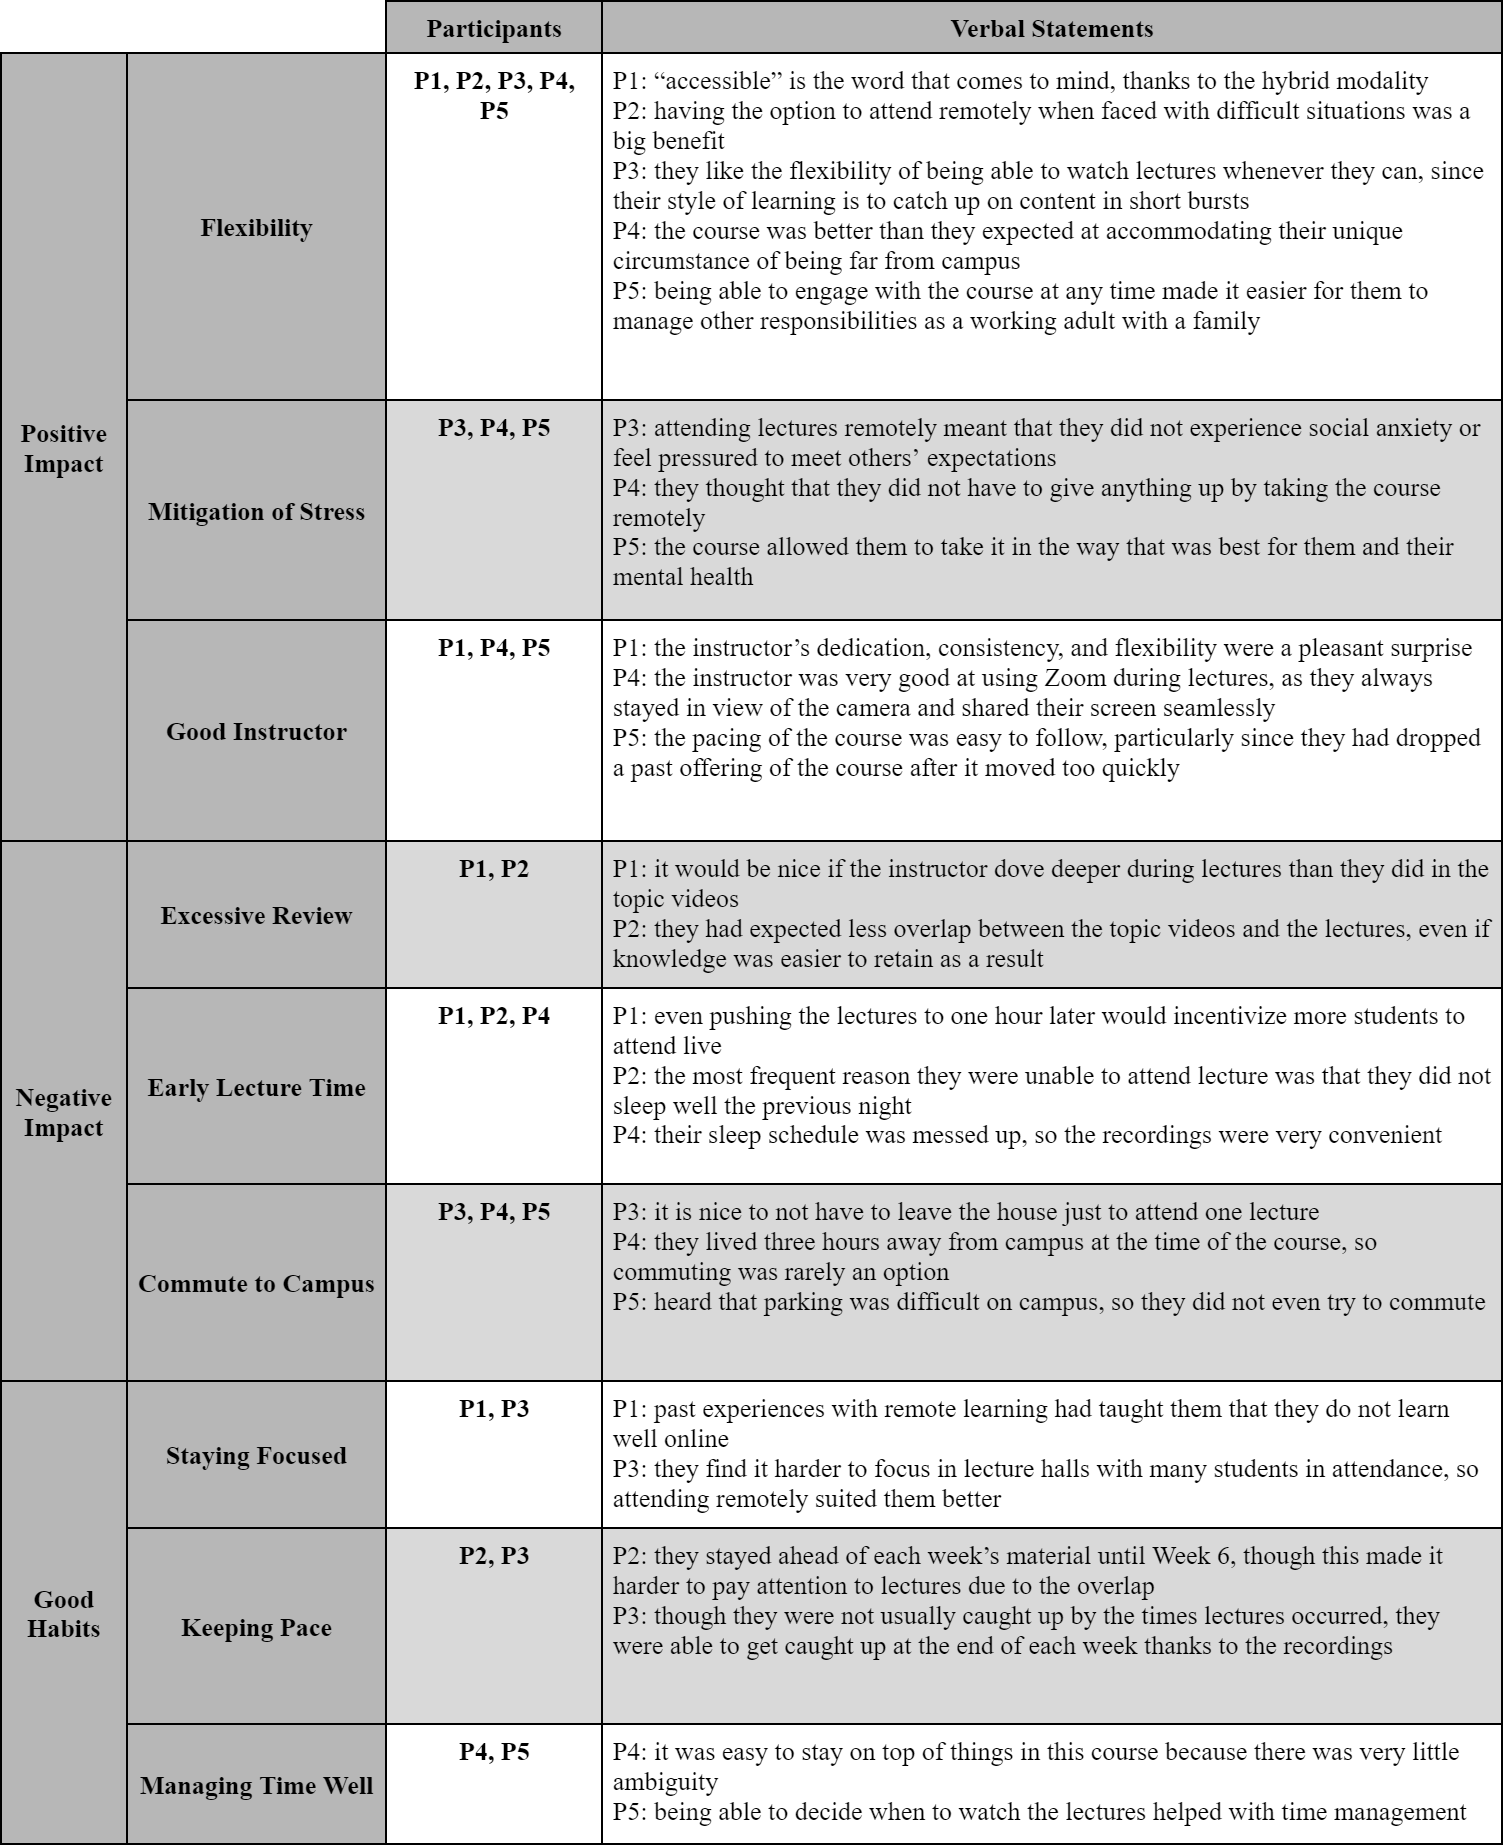
\includegraphics[width= 16cm]{figures/interview_response_codes.png}
    \label{tab:interview_response_codes}
\end{table}

\section{Identified Factors}

With the information that was provided to us by the interview participants and the responses that we gathered through the course surveys, we were able to identify the following five primary factors that impact the modality and frequency of a student’s lecture attendance in a hybrid course.

\subsection{Personal Preference}

99.0\% of pre-course survey respondents stated that they had used the remote conferencing tool Zoom in one of their previous courses, meaning that very few students had their first experience with remote learning at the time of the study. As a result, many students had already determined which modality they would prefer, in-person or remote, before they had even started the course. When asked which modality they would prefer if the course had been offered as solely in-person or solely remote, 39.0\% chose in-person, 39.7\% chose remote, and 21.3\% stated no preference either way. As shown in Table \ref{tab:attendance-initial-preference}, students who said that they would prefer an in-person course were much more likely to attend the lectures in person during the first half of the course. When P1 was asked why they preferred to learn in person, they explained that their fully remote senior year of high school had demonstrated to them that they are unable to engage properly with their schoolwork without “seeing it in front of [them] and having fewer distractions.” They always tried to attend the lectures live so that they could learn important information without having to watch the lecture recordings, which they rarely did out of dislike for the format. On the opposite end of the spectrum, P5’s discovery that they could engage with the lectures at any time throughout the week through the recordings was instrumental in their ability to succeed in the course; they mentioned that they had dropped the course in the past due to feeling unprepared for the pace at which they would need to learn.

\subsection{Early Expectations}

All five interviewees had entered the course with a general idea of how they would be attending each of the lectures. Of them, the in-person and hybrid attendees (P1 and P2) were let down by the in-person lecturing experience they received, while the remote and asynchronous attendees (P3, P4, and P5) found that the lectures surpassed their expectations for what a remote course could offer them. The differences in their expectations could be explained by the high standards that the students had for in-person courses and the relatively lower standard for remote courses that they had developed during the COVID-19 pandemic: P4 stated that several remote courses they had taken in the past had clearly been designed for in-person attendees, and they asserted that “some professors can’t teach online and provide a cohesive experience at the same time.” This course had been the first to show P4 that it could be achieved successfully at a large scale. And based on the survey data depicted in Table \ref{tab:attendance-initial-preference}, it appears that they were not alone in this regard: over half of the students who submitted responses to both the pre-course and the end-of-course surveys attended lectures asynchronously as they reached the end of the course, denoting a large shift away from the in-person end of the modality spectrum. Though most fully in-person courses in the department also regularly experience a drop-off in attendance over time, the way that this course was able to provide a comparable experience to remote, asynchronous, and non-attendees surprised students: when asked about the ways in which the course differed from their expectations in an optional question on the end-of-course survey, 7 of the 32 respondents took the opportunity to simply say that the hybrid model had far surpassed what they had anticipated. One student noted that they were “honestly surprised that this hybrid structure isn't the standard for courses in the department.”

\subsection{Conflicting Circumstances}

The interviewees who attended remotely or asynchronously each cited physical location as a reason why they would not be able to attend lectures in person: P3 stated that they enjoyed not having to leave their house just to attend the one lecture they had on Mondays, Wednesdays, and Fridays, while P4 and P5 both resided a long distance from campus and would not be able to attend without conducting a lengthy commute. Given that the course had been advertised beforehand as a hybrid course, these individuals had knowingly enrolled in the course with the intent to take advantage of the remote and asynchronous modalities from a distant location, limiting their available options from the very beginning. As can be seen in Figure \ref{fig:remote_attendance_reasons}, around 15\% of respondents to the mid-course and end-of-course survey cited physical distance from their on-campus residences as a reason for their inability to attend lectures in person, while a further 5\% stated that they resided off-campus and did not have a method of transportation to arrive at the location of the lectures. However, a much more common reason why students were unable to attend in person was the timing of the lectures: over half of the respondents to the mid-course survey cited the early lecture times as a factor in their decision to not attend in-person lectures, while just under half of the end-of-course survey respondents gave the same reasoning. The interviewees who had attended in-person lectures, P1 and P2, both spoke about how the earliness of the lectures had negatively impacted their ability to attend consistently, with the latter mentioning that their inconsistent sleep schedule occasionally made in-person attendance an impossibility. This would indicate that, while an inconvenient location rules out in-person attendance entirely for individuals who plan to take lectures from the start, inconvenient timing will drastically decrease the motivation to attend in-person lectures in those who would otherwise be able to do so.

\subsection{Flexible Format}

Despite the difference in the modalities that were experienced by each of the interviewees, all of them were similarly impacted by the flexibility afforded to them by the dual-modality structure of the course. P1 and P2 both attested that, despite their frequent in-person attendance, they were unconcerned about missing the occasional lecture because they were able to attend remotely or asynchronously through the lecture recordings. P3, P4, and P5 all claimed that having the ability to absorb the material at their own pace was beneficial to their time management for the course; P5, having developed self-discipline in their past as a member of the military, spoke highly about the level of control that the course granted them over their education and its removal of stresses unrelated to the course, such as the lengthy commute and the availability of on-campus parking. This sentiment was echoed in 17 of 24 responses to an optional question on the mid-course survey: commutes, early lectures, and the inability to find parking were the factors most frequently cited by students when they were asked to explain why they did not attend in person. When one can join a lecture at the press of a button or the click of a link, or watch a recording later on EdStem, it was difficult for them to justify waking up early and dealing with the hassle of their commute. As seen in Table \ref{tab:attendance-modalities-tab}, the percentage of students who attended lectures in person dropped from 28.5\% in the first half of the course to 16.8\% in the second half, and synchronous attendees collectively dropped from 48.6\% to 25.0\% during the same time frame.

\subsection{Insightful Instructor}

Another commonality among participants was their attestation that the expertise of the instructor motivated them to continue engaging with the lectures in some form or another. Both P1 and P4 were impressed by the instructor’s ability to split their attention across two different modalities at the same time, and they praised the level of familiarity that the instructor had with utilizing Zoom during lectures. P1, being an in-person attendee, observed that the instructor always made sure to verbally repeat their questions before answering them for the benefit of the remote attendees, and they felt that this prevented one of the main drawbacks of attending a lecture through Zoom that many other instructors are not even aware of. P4, being a remote attendee, noted that they could always see and hear the instructor because they kept within the camera frame and spoke directly into the microphone, a feat that they had never seen in a remote course before this one. Despite utilizing different modalities, both of these participants were able to notice these details, and both were incentivized to attend lectures more often as a result. Three respondents to an optional question on the end-of-course survey also took note of the instructor’s organizational and presentational skills, with one musing that they “wish [their] other professors could learn from this class.”

\vspace{2cm}
\chapter{Discussion}

\section{Interpretation of Results}

Through the pre-course survey, we were able to gather demographic data on the students of the course and learn their justifications for enrolling in each of the sections of the course, as well as their overall modality preference. In turn, the mid-course and end-of-course surveys provided us with a way to classify students by their modality of lecture attendance, as well as the reasons that either helped or hindered students when they decided whether to attend lectures in person. By analyzing the responses we gathered through these surveys, we came to the following conclusions for our research questions.

\subsection{Attendance plans are impacted by class standing, less so by gender.}

By stratifying the pre-course survey data, we find that a student's class standing had an impact on their feelings towards in-person and remote modalities: as Figure \ref{fig:modality_preference} shows, students of higher class standings were proportionately more likely to prefer a remote offering over an in-person offering, while the opposite was true of lower class standings. Figure \ref{fig:inperson_enrollment_reasons} shows that second-year undergraduate students who were enrolled in the in-person section were more likely to indicate that they would be on campus when the lectures took place,  and Figure \ref{fig:remote_enrollment_reasons} shows that undergraduate students in their fifth year or beyond were by far the most likely remote enrollees to indicate that they would not be able to get to campus. This may be due, in part, to the fact that on-campus housing is only guaranteed for undergraduate students until the end of their second year, meaning that undergraduate students beyond that point must seek out off-campus options that require them to commute to campus. Further supporting this hypothesis is the fact that graduate students, who are also guaranteed on-campus housing, were not likely to report that they would be unable to get to campus.

Meanwhile, gender appeared to have a less pronounced impact on students' attendance plans at the beginning of the course. Figure \ref{fig:remote_enrollment_reasons} shows that the female students enrolled in the remote section were proportionally less likely to prefer remote modalities than male students. However, only a slightly higher percentage of female students were enrolled in the in-person section. While the reason for this discrepancy is not clearly defined and warrants further study, one interviewee who identified as female offered a possible explanation: they stated that their past experiences with computer science courses had been that male students were the most confident and outspoken, while female students were more hesitant to answer questions during lectures for fear of being wrong. Another female student shared that they had experienced certain uncomfortable interactions with male classmates in the past when attending lectures in-person, and they had thus been more inclined to engage with the course remotely from the start. It appears that the degree to which the field of computer science is male-dominated may have discouraged some female students from considering the in-person modality of the course in spite of their lack of enjoyment for remote learning.

However, unlike class standing and gender, race did not appear to have an impact on students' plans for attendance at the beginning of the course. This may have been due to the fact that the course was heavily skewed towards Asian and White individuals, with members of minority groups not being nearly as represented in our study. This is another potential factor that would benefit from further study, and other researchers would do well to observe a course that has a diverse population of individuals should they conduct a deeper investigation on the impact of race on modality preference.

\subsection{Convenience is key.}

When it came time for students to decide whether to attend lectures in person, they were deterred most often by the early time at which lectures took place: Figure \ref{fig:remote_attendance_reasons} demonstrates how approximately half of the remote, asynchronous, and non-attendees of the course considered the earliness of the lectures to be a factor in their decision to not attend in-person lectures. This, along with the need to commute and the inability to find parking on campus, were all common obstacles mentioned by survey respondents. Often, just one of these factors had been enough to deter a student from heading to the on-campus location from which lectures were held, particularly since remote and asynchronous modalities were accessible from any other location. Interviewees and survey respondents who recounted that they had experienced poor sleep schedules during their time with the course also mentioned that they were also not as motivated to engage with the remote modality for the lectures, choosing to watch the lecture recordings at a later point in the day rather than deprive themselves of more sleep. From these observations, we can conclude that convenience is viewed by many students to be the strongest factor that determines their modality of attendance, even more so than personal preference. Even if students believe that in-person lectures provide a higher-quality educational experience, a course that provides no extrinsic incentive for in-person attendance will likely see few in-person attendees if even one inconveniencing factor is at play.

This desire for convenience extended beyond just the in-person lectures, however: as one respondent to the end-of-course survey put it, having the same content be available across the topic videos, the online textbook, and the lectures made it so that students were less likely to attend lectures remotely as well. Given that the number of remote attendees decreased at a faster rate than the number of in-person attendees, this would imply that students who started to attend remotely eventually found asynchronous recordings to be the most convenient modality of the three, while in-person attendees were more likely to prioritize engagement over convenience. The convenience of being able to access well-designed course material at one's own pace further compounded some students' desires to engage with the course without attending the lectures. From a logistical perspective, having multiple methods through which students can learn about course concepts increases the likelihood that their knowledge of the material will be reinforced; however, it is easy to see how a student can perceive these methods to be redundant and prioritize the most convenient option over all others, even if that method does not allow them to follow up on their misunderstandings and ask clarifying questions as a lecture would. Thus, we hypothesize that while students in HyFlex courses tend to drift towards remote and asynchronous modalities, a flipped HyFlex course is more likely to have students forego synchronous attendance entirely.

\section{Call to Action}

Through the surveys and the follow-up interviews, we identified five main factors that affect the modality through which students attend lectures: personal preference, early expectations, conflicting circumstances, a flexible format, and an insightful instructor. Of the five, the first three were factors that students had already developed by the time they had started the course, meaning that they could not reasonably be changed by those who are managing the course. However, the last two are entirely within the control of the course administrators, particularly the final factor regarding instructor insight. As a result, this section will focus on providing suggestions to instructors and their institutions that offer future HyFlex courses on the ways in which they might be able to influence the modalities through which students attend their lectures. We will not concern ourselves with factors that are out of the control of instructors and instead focus on the aspects that would most benefit from their input.

\subsection{Clearly communicate course logistics.}

As indicated by the high percentage of enrollees in the remote section of the course who did so because the in-person section was full, the fact that both sections of enrollment were functionally identical and met the same course requirements was not well advertised to students prior to the course. Even by the end of the course, four survey respondents expressed that they had not attended lectures in person due to being enrolled in the remote section, showing a lack of communication on behalf of the instructors of the course. Had the department's administration instead offered the course under a single section, the freedom to choose any attendance modality may have come across more clearly to these students. It should be noted that the offering of the course that we observed in our study was the debut of a new course code, which may become less confusing to students of future offerings. Nevertheless, in a course that has multiple modalities through which instructors must communicate with their students, it is imperative that important details about the course are established even before the first lecture is held.

\subsection{Make synchronous lectures more accessible.}

When asked about the reasons why they had not attended lectures in person, two of the remote and asynchronous attendees expressed that they preferred in-person over remote when directly comparing the two modalities, and one even stated that they knew that they would learn better in an in-person environment. However, these respondents faced obstacles that made it difficult for them to choose in-person over remote on most occasions. Factors such as the lengthy commute and limited access to parking exacerbated the rate of decline for in-person attendance to the point where only 16.8\% of students attended lectures in person during the second half of the course. However, the most common of these obstacles was the fact that the lectures were scheduled at 9:00 AM, which these respondents found to be too early, and this even discouraged remote attendees from attending synchronously. As previously mentioned in the Results section, lecture attendance almost always decreases over time in the courses offered by the department, and the fact that students were able to still attend asynchronously at any time and place was cited by many to be the largest benefit of a HyFlex course over previous courses that they had taken. However, the downside of flexibility is that it may discourage students from taking the action that will most benefit their own learning in favor of the one that is most convenient for them.

As a result, instructors would do well to make synchronous modalities more accessible in the ways that are available to them. One possible way to circumvent an early lecture time, for instance, would be to hold other events later in the day that allow students to engage with the course material outside of lectures, such as office hours or tutoring hours. If these events are held in more convenient locations for students, that could also benefit those who struggle to commute and find parking, since those students would have more opportunities to commute to locations that demand a shorter commute or have more available parking spaces. Importantly, the nature of a HyFlex course makes it so that dedicating more attention towards prospective in-person attendees should not have a negative impact on those who would attend remotely or asynchronously regardless of accessibility. The increase in accessibility for prospective in-person attendees should not come at the expense of those using other modalities, nor should in-person attendees receive benefits that are inaccessible to other types of attendees. Meanwhile, institutions should reconsider scheduling HyFlex courses at times that are inconvenient for students, because this is likely to result in most students treating the course as if it were entirely online. The choice, then, is whether it would be more appropriate to offer those courses as online-only courses or to hold them at times that will allow for a much higher number of students to attend synchronously.

\subsection{Practice teaching across multiple modalities.}

Though the interview participants experienced the course through different modalities, one observation that was made by both in-person and remote attendees was that the instructor for the course was experienced in teaching through multiple modalities at once. Their knowledge of Zoom as a teaching tool enabled them to effectively lead a discussion simultaneously across modalities, even as they received questions in person and read comments sent through the online chat. This resulted in an environment in which both in-person and remote attendees felt heard, and this was cited by many survey respondents as something that motivated them to attend lectures synchronously. It is clear that effective management of the modalities results in increased engagement from students, so instructors who are less experienced with the balancing act of HyFlex instruction should take the time to practice doing so. One specific skill that should be focused on is the ability to verbally repeat questions asked by in-person attendees for the benefit of remote and asynchronous attendees and verbally repeat chat messages sent by remote attendees for the benefit of in-person and asynchronous attendees. Instructors should seek out resources that can help them develop this skill; for instance, the Teaching + Learning Commons at the University of California San Diego offers training sessions for instructors on how to use new technologies for their courses. Institutions, in turn, should consider investing in the development of such resources for their instructors, especially if they have yet to do so. Instructors can also have the course's TAs and tutors assist them by facilitating the discussions that take place online, such as by responding to questions that were sent through the chat or guiding students verbally during break-out discussion sections.

\section{Limitations and Future Work}

\subsection{Underrepresented Groups}

There were a few aspects of our study that could use some refinement in future iterations. Most glaringly, as mentioned previously in our discussions of race and gender, there were not as many underrepresented groups in our study as we would have liked due to the demographics of the course being heavily skewed towards Asian, White, and male students. Though we were able to gain further insight on the experiences of female students from the interviews and optional short answer responses, the homogeneity of the student body increases the likelihood that certain observations made in our study will not apply as directly to students of underrepresented groups. Future studies that decide to investigate that direction further should take care to observe a course with a more even distribution of race and gender across its students.

\subsection{Courses with Different Logistics}

In addition, this study was centered around a new offering of a specific course taught by a single instructor at a single institution, which could limit the applicability of our findings to some degree. For example, another course could be taught by multiple instructors and thus provide multiple different opportunities for students to attend lectures live, which may increase the number of synchronous attendees. In addition, the course that we observed is one of the first upper-division courses that are taken by students of the department; it is entirely possible that students in an introductory course or one of the later upper-division courses would require more extrinsic motivators or additional assistance in order to keep being motivated to attend lectures. There are also factors related to both the subject and the students that should be considered: would a theory course with fewer coding-intensive assignments see higher or lower attendance counts than the ones that we observed? If so, which modalities would differ most in this regard? On the other hand, perhaps the recency of the COVID-19 pandemic, which forced many students to enroll in online courses, resulted in students' desires to attend in-person courses to be higher than they would be otherwise. These additional considerations only scratch the surface at the number of possible directions that future studies on HyFlex courses could take.

\subsection{Data Collection Methods}

The methods through which in-person attendance was measured were somewhat imprecise. Pictures and self-reported attendance counts could only capture a proportion of the full group of in-person attendees in the course: the former could not account for individuals who joined the in-person lectures after they began (such as the individual who attended remotely while they conducted their commute to the lecture hall), while the latter was subject to sampling bias and was more representative of those who attended lectures due to the in-class announcements that were made upon the release of the surveys. Because these metrics were less precise than our remote attendance counts, the classifications we designed for attendance types were not as consistent as they could have been, and the overall strength of our data analysis suffered as a result. In the interest of providing a fair experience for students across all modalities, we did not use any methods of tracking the in-person attendance of individual students that impacted grades, such as participation points; however, future studies may be able to gather in-person attendance data through a more efficient method, which would in turn lead to more accurate classifications for attendance types and a subset that is a more accurate representation of the entire course.

\subsection{Directions for Further Research}

The work presented in this paper invites institutions to more intelligently design their flipped HyFlex courses, especially when the needs of students could differ depending on the specific flipped HyFlex course that they are enrolled in. However, there is still much to learn about the intersection between flipped courses and HyFlex courses, and we encourage others to conduct their own studies on courses that combine the two models. Apart from the aforementioned limitations to our study, there are a number of aspects that could be investigated further by researchers in future studies.

One potential direction for further research would be to implement the suggested changes presented above in another flipped HyFlex course and measure whether they have an impact on the utilization level of each attendance modality, particularly in-person attendance. Other researchers may find additional factors impacting attendance that we could not, either due to the limited scope of our study or the setting in which our study took place.

It should also be noted that our study took place only a few years after the COVID-19 pandemic altered the educational paths of many students in institutions around the world. There is reason to believe that the recency of such an impactful event may have caused our data to vary noticably from what future studies may obtain from their inverted HyFlex courses, and that potential discrepancy further supports our call for more research to take place on this topic.

In addition, the only components of our course that were offered in multiple modalities were the lectures and the discussion sections. Other courses may choose to offer tutoring hours or office hours across in-person and remote modalities as well, and the effect that such an addition has on students is a worthy topic for investigation.

We also invite future researchers to make their own observations on flipped HyFlex courses and further investigate the nature of both flipped classrooms and HyFlex. It is our belief that a deeper understanding of course designs like flipped classroom and HyFlex could eventually lead to the development of an educational model that, much like HyFlex itself, brings together various aspects of other models to form a whole that is greater than the sum of its parts.
% \chapter{Conclusion}

%% APPENDIX
\appendix
\chapter{Pre-Course Survey}\label{sec:appendix_a}
\begin{enumerate}
    \item Which of the following CSE courses have you taken at UCSD? \textit{(Checkboxes, select one or more)}
    \begin{enumerate}
        \item CSE 8A. Introduction to Programming and Computational Problem-Solving I
        \item CSE 8B. Introduction to Programming and Computational Problem-Solving II
        \item CSE 11. Introduction to Programming and Computational Problem-Solving: Accelerated Pace
        \item CSE 12. Basic Data Structures and Object-Oriented Design
        \item CSE 15L. Software Tools and Techniques Laboratory
        \item CSE 20. Discrete Mathematics
        \item CSE 21. Mathematics for Algorithms and Systems
        \item CSE 30. Computer Organization and Systems Programming
        \item Other
    \end{enumerate}

    \item Which of the following learning tools have you used in a previous course? \textit{(Checkboxes, select one or more)}
    \begin{enumerate}
        \item Ed/EdStem (digital learning platform)
        \item Piazza (class discussion platform)
        \item Autograder (tutor queue platform)
        \item Stepik (online textbook platform)
        \item Zoom (conference call platform)
        \item None of the above
        \item Other
    \end{enumerate}

    \item In which section of the course are you officially enrolled? \textit{(Multiple Choice, choose one; the response to this question determined which section of the survey would come next)}
    \begin{enumerate}
        \item CSE 100 (in-person)
        \item CSE 100R (remote)
    \end{enumerate}

\noindent \textbf{CSE 100 (IN-PERSON)}

    \item Why did you choose to enroll in the in-person section? \textit{(Checkboxes, select one or more)}
    \begin{enumerate}
        \item I prefer to learn in an in-person setting.
        \item It is easier for me to learn in an in-person setting.
        \item I will already be on campus on those days, so it is more convenient.
        \item I am concerned that I will be unable to focus if I attend remotely.
        \item None of the above
        \item Other
    \end{enumerate}

    \item On average, how often do you plan to attend the in-person lectures? \textit{(Multiple Choice, choose one)}
    \begin{enumerate}
        \item Less than once a week
        \item Once a week
        \item Twice a week
        \item As often as possible
        \item Not sure yet
    \end{enumerate}

\noindent \textbf{CSE 100R (REMOTE)}

    \item Why did you choose to enroll in the remote section? \textit{(Checkboxes, select one or more)}
    \begin{enumerate}
        \item I prefer to learn in a remote setting.
        \item It is easier for me to learn in a remote setting.
        \item I am unable to get to campus on those days, so it is more convenient.
        \item I am concerned for my health during the ongoing COVID-19 pandemic.
        \item The in-person section was full.
        \item None of the above
        \item Other
    \end{enumerate}

    \item Do you plan to attend an in-person lecture at some point? \textit{(Multiple Choice, choose one)}
    \begin{enumerate}
        \item Yes
        \item No
        \item Not sure yet
    \end{enumerate}

\noindent \textbf{ALL RESPONDENTS}

    \item How many units are you enrolled in for this quarter? \textit{(Short Answer, numerical)}

    \item Excluding CSE 100/100R, how many of your units for this quarter are for remote courses? \textit{(Short Answer, numerical)}

    \item If CSE 100 was only offered as either an in-person or a remote course, which modality would you prefer? \textit{(Multiple Choice, choose one)}
    \begin{enumerate}
        \item Between the two, I would prefer in-person.
        \item Between the two, I would prefer remote.
        \item I have no preference.
    \end{enumerate}

    \item What is your current class standing? \textit{(Multiple Choice, choose one)}
    \begin{enumerate}
        \item 1st Year (Undergrad)
        \item 2nd Year (Undergrad)
        \item 3rd Year (Undergrad)
        \item 4th Year (Undergrad)
        \item 5th+ Year (Undergrad)
        \item Masters/PhD Student
        \item Other
    \end{enumerate}

    \item Did you enter UCSD as a transfer student from another (two-year or four-year) college or university? \textit{(Multiple Choice, choose one)}
    \begin{enumerate}
        \item Yes
        \item No
        \item N/A (I am a Masters/PhD student)
    \end{enumerate}

    \item Which gender do you most identify as? \textit{(Multiple Choice, choose one)}
    \begin{enumerate}
        \item Male
        \item Female
        \item Non-binary
        \item Prefer not to answer
        \item Other
    \end{enumerate}

    \item Do you identify as LGBTQIA+? \textit{(Multiple Choice, choose one)}
    \begin{enumerate}
        \item Yes
        \item No
        \item Prefer not to answer
        \item Other
    \end{enumerate}

    \item How would you describe yourself? \textit{(Checkboxes, select one or more)}
    \begin{enumerate}
        \item White (e.g. German, Irish, English, Italian, Polish, French)
        \item Black or African American (e.g. African American, Jamaican, Haitian, Ethiopian)
        \item Asian (e.g. Chinese, Filipino, Vietnamese, Korean, Japanese, Asian Indian)
        \item American Indian or Alaska Native (e.g. Navajo nation, Blackfeet tribe, Mayan, Aztec)
        \item Middle Eastern or North African (e.g. Lebanese, Iranian, Egyptian, Syrian, Moroccan)
        \item Native Hawaiian or Other Pacific Islander (e.g. Samoan, Chamorro, Tongan, Fijian)
        \item Prefer not to answer
        \item Other
    \end{enumerate}

    \item Are you of Hispanic, Latino, or Spanish origin? \textit{(Multiple Choice, choose one)}
    \begin{enumerate}
        \item Yes
        \item No
        \item Prefer not to answer
    \end{enumerate}
\end{enumerate}
\chapter{Mid-Course Survey}\label{sec:appendix_b}
\begin{enumerate}
    \item What is your current major? \textit{(Checkboxes, select one or more)}
    \begin{enumerate}
        \item Computer Science
        \item Computer Engineering
        \item Data Science
        \item Cognitive Science
        \item Mathematics-Computer Science
        \item Bioengineering w/ Specialization in Bioinformatics
        \item Biology w/ Specialization in Bioinformatics
        \item Chemistry and Biochemistry w/ Specialization in Bioinformatics
        \item Interdisciplinary Computing and the Arts (ICAM)
        \item Other
    \end{enumerate}

    \item In which section of the course are you officially enrolled? \textit{(Multiple Choice, choose one)}
    \begin{enumerate}
        \item CSE 100 (in-person)
        \item CSE 100R (remote)
    \end{enumerate}

    \item Do you live on campus or off campus? \textit{(Multiple Choice, choose one)}
    \begin{enumerate}
        \item On campus
        \item Off campus
    \end{enumerate}

    \item Excluding Lecture 0, approximately how times did you attend a lecture, in person OR remotely, by the end of Week 5? \textit{(Multiple Choice, choose one)}
    \begin{enumerate}
        \item 0 times
        \item 1 to 5 times
        \item 6 to 10 times
        \item 11 to 15 times
    \end{enumerate}

    \item Excluding Lecture 0, approximately how many times did you attend a lecture IN PERSON by the end of Week 5? \textit{(Multiple Choice, choose one; the response to this question determined which section of the survey would come next)}
    \begin{enumerate}
        \item 0 times
        \item 1 to 5 times
        \item 6 to 10 times
        \item 11 to 15 times
    \end{enumerate}

\noindent \textbf{HYBRID, IN-PERSON ATTENDEES}

    \item Which of the following reasons have enabled you to keep attending lectures in person? \textit{(Checkboxes, select one or more)}
    \begin{enumerate}
        \item I prefer to learn in an in-person setting.
        \item It is easier for me to learn in an in-person setting.
        \item I am already near the lecture hall on those days, so it is more convenient.
        \item I enjoy the level of engagement involved in attending lectures in person.
        \item I feel more involved in the class community when I attend lectures in person.
        \item I live on/near campus.
        \item None of the above
        \item Other
    \end{enumerate}

    \item (Optional) Please elaborate on your response to the previous question. \textit{(Free Response)}

\noindent \textbf{REMOTE, ASYNCHRONOUS, NON-ATTENDEES}

    \item Which of the following reasons have prevented you from attending lectures in person? \textit{(Checkboxes, select one or more)}
    \begin{enumerate}
        \item I prefer to learn in a remote setting.
        \item It is easier for me to learn in a remote setting.
        \item I am concerned for my health during the ongoing COVID-19 pandemic.
        \item I do not have a method of transportation that allows me to get to campus.
        \item I have a scheduling conflict that prevents me from attending lectures live.
        \item The lecture hall is too far from my on-campus residence.
        \item The scheduled lecture time is too early in the day.
        \item None of the above
        \item Other
    \end{enumerate}

    \item (Optional) Please elaborate on your response to the previous question. \textit{(Free Response)}

\noindent \textbf{ALL RESPONDENTS}

    \item Approximately how many times did you attend a discussion section IN PERSON by the end of Week 5? \textit{(Short Answer, numerical from 0 to 5)}

    \item How frequently did you do the following by the end of Week 5? \textit{(Likert scale: 1–5 where 1 was labeled as ``Never'' and 5 was labeled as ``Several times a week'')}
    \begin{enumerate}
        \item watch a topic video on EdStem
        \item watch a lecture recording on EdStem
        \item watch a discussion section recording on EdStem
        \item go to tutor lab hours on Autograder
        \item go to TA office hours on Zoom
        \item submit a post to the EdStem Discussion Board
        \item read another student's post on the EdStem Discussion Board
        \item ask a question in the CSE 100/100R Discord server
    \end{enumerate}

    \item Would you be more likely to go to the tutor lab hours if they were held in person in the CSE Basement, in addition to being held over Zoom? \textit{(Multiple Choice, choose one)}
    \begin{enumerate}
        \item Yes
        \item No
        \item Not sure
    \end{enumerate}

    \item Would you be more likely to go to the TA office hours if they were held in person in the CSE Basement, in addition to being held over Zoom? \textit{(Multiple Choice, choose one)}
    \begin{enumerate}
        \item Yes
        \item No
        \item Not sure
    \end{enumerate}

    \item (Optional) What suggestions do you have for potential resources that could be made available in future offerings of CSE 100/100R? \textit{(Free Response)}

    \item Would you be willing to participate in a 30-minute-long follow-up interview over Zoom on your thoughts about CSE 100/100R? We would love to hear what you have to say! \textit{(Multiple Choice, choose one)}
    \begin{enumerate}
        \item Yes
        \item No
    \end{enumerate}
\end{enumerate}
\chapter{End-of-Course Survey}\label{sec:appendix_c}
\begin{enumerate}
    \item Approximately how times did you attend a lecture, in person OR remotely, from the start of Week 6 to the end of Week 10? (If you are taking this survey before the final lecture, you may provide an estimate.) \textit{(Multiple Choice, choose one)}
    \begin{enumerate}
        \item 0 times
        \item 1 to 5 times
        \item 6 to 10 times
        \item 11 to 15 times
    \end{enumerate}

    \item Approximately how times did you attend a lecture IN PERSON from the start of Week 6 to the end of Week 10? (If you are taking this survey before the final lecture, you may provide an estimate.) \textit{(Multiple Choice, choose one; the response to this question determined which section of the survey would come next)}
    \begin{enumerate}
        \item 0 times
        \item 1 to 5 times
        \item 6 to 10 times
        \item 11 to 15 times
    \end{enumerate}

\noindent \textbf{HYBRID, IN-PERSON ATTENDEES}

    \item Which of the following reasons have enabled you to keep attending lectures in person? \textit{(Checkboxes, select one or more)}
    \begin{enumerate}
        \item I prefer to learn in an in-person setting.
        \item It is easier for me to learn in an in-person setting.
        \item I am already near the lecture hall on those days, so it is more convenient.
        \item I enjoy the level of engagement involved in attending lectures in person.
        \item I feel more involved in the class community when I attend lectures in person.
        \item I live on/near campus.
        \item None of the above
        \item Other
    \end{enumerate}

    \item (Optional) Please elaborate on your response to the previous question. \textit{(Free Response)}

\noindent \textbf{REMOTE, ASYNCHRONOUS, NON-ATTENDEES}

    \item Which of the following reasons have prevented you from attending lectures in person? \textit{(Checkboxes, select one or more)}
    \begin{enumerate}
        \item I prefer to learn in a remote setting.
        \item It is easier for me to learn in a remote setting.
        \item I am concerned for my health during the ongoing COVID-19 pandemic.
        \item I do not have a method of transportation that allows me to get to campus.
        \item I have a scheduling conflict that prevents me from attending lectures live.
        \item The lecture hall is too far from my on-campus residence.
        \item The scheduled lecture time is too early in the day.
        \item The ongoing TA strike has made it harder to come to campus.
        \item None of the above
        \item Other
    \end{enumerate}

    \item (Optional) Please elaborate on your response to the previous question. \textit{(Free Response)}

\noindent \textbf{ALL RESPONDENTS}

    \item How frequently did you do the following by the end of Week 5? \textit{(Likert scale: 1–5 where 1 was labeled as ``Never'' and 5 was labeled as ``Several times a week'')}
    \begin{enumerate}
        \item watch a topic video on EdStem
        \item watch a lecture recording on EdStem
        \item watch a discussion section recording on EdStem
        \item go to tutor lab hours on Autograder
        \item go to TA office hours on Zoom
        \item submit a post to the EdStem Discussion Board
        \item read another student's post on the EdStem Discussion Board
        \item ask a question in the CSE 100/100R Discord server
    \end{enumerate}

    \item How frequently did you do the following by the end of Week 5? \textit{(Likert scale: 1–5 where 1 was labeled as ``Very unhelpful'' and 5 was labeled as ``Very helpful''; another option was ``I never used this resource.'')}
    \begin{enumerate}
        \item topic videos on EdStem
        \item lecture recordings on EdStem
        \item discussion recordings on EdStem
        \item tutor lab hours on Autograder
        \item TA office hours on Zoom
        \item posts on the EdStem Discussion Board
        \item questions in the Discord server
    \end{enumerate}

    \item After learning about each of the following topics in CSE 100/100R, how much did you understand them? \textit{(Likert scale: 1–5 where 1 was labeled as ``What is this?'' and 5 was labeled as ``I fully understood this topic.'')}
    \begin{enumerate}
        \item C++ Syntax \& Iterators
        \item Time \& Space Complexity
        \item Binary Search Trees (BSTs)
        \item Treaps \& Randomized Search Trees (RSTs)
        \item AVL Trees \& Red-Black Trees
        \item Multiway Tries (MWTs)
        \item Ternary Search Trees (TSTs)
        \item Hash Tables \& Hash Maps
        \item Collision Resolution Strategies
        \item Bloom Filters \& Count-Min Sketches
        \item Aho-Corasick Automatons
        \item Suffix Arrays
        \item Burrows-Wheeler Transforms (BWTs)
        \item Huffman Coding
        \item Bitwise Input/Output
        \item Graphs \& Dijkstra's Algorithm
        \item Minimum Spanning Trees
        \item Disjoint Sets
    \end{enumerate}

    \item If you were able to go back in time, would you choose to enroll in this offering of CSE 100/100R again? \textit{(Multiple Choice, choose one)}
    \begin{enumerate}
        \item Yes, I would enroll in CSE 100.
        \item Yes, I would enroll in CSE 100R.
        \item No, I would not enroll in CSE 100/100R.
        \item I am unsure.
    \end{enumerate}

    \item (Optional) In what ways did CSE 100/100R differ from your expectations for the course? \textit{(Free Response)}

    \item (Optional) What suggestions do you have for changes to CSE 100/100R that would make the course more accessible for different groups of students? \textit{(Free Response)}
\end{enumerate}
\chapter{Follow-Up Interviews}\label{sec:appendix_d}

\begin{enumerate}
    \item You mentioned in the initial course survey that, if given the choice between in-person and remote options for this course, you would prefer in-person/remote. What factors affected your preference? Has your preference changed after enrolling in this course?
    \item You also mentioned in the survey that you chose to enroll in the in-person/remote section because \rule{1cm}{0.15mm}. Do you stand by these reasons now that you have completed this course? How accurately do you feel you predicted your experiences with the course?
    \item What were your expectations going into this course for how much you would interact with the in-person aspects of the course (i.e. lectures, discussions)? How about the remote aspects (i.e. lab hours, office hours, EdStem discussion board)?
    \item Were there any unique benefits or challenges you found in this course that exist due to the dual-modality nature of the course?
    \item What are some strategies that you have used in this course due to the dual-modality nature of the course?
    \item What are some ways that you believe the course could incentivize your engagement with the course resources, both in-person and remote?
    \item What advice would you provide a student who is about to enroll in this course, as it is in its current offering?
\end{enumerate}


%% END MATTER
\bibliographystyle{acm}
\bibliography{bib}
\singlespace  %to force bibilography environment to use single spacing for each entry 
              %double spacing between entries remains
\end{document}

